\documentclass[master=elt,masteroption=eg,english]{kulemt}
\setup{% Verwijder de "%" op de volgende lijn bij UTF-8 karakterencodering
  %inputenc=utf8,
  title={Learning comfort objective from lane change demonstrations for optimal control},
  author={Stijn Staring},
  promotor={Prof.\,dr.\,ir.\ Jan Swevers},
  assessor={Prof.\,dr.\,ir.\ Bert Pluymers\and Prof.\,dr.\,ir.\ Herman Bruyninckx},
  assistant={Dr.\,ir.\ Son Tong}}
% DENK ERAAN OM DE MASTER OPTIE AAN TE PASSEN OP HET EINDE!
% Verwijder de "%" op de volgende lijn als je de kaft wil afdrukken
%\setup{coverpageonly}
% Verwijder de "%" op de volgende lijn als je enkel de eerste pagina's wil
% afdrukken en de rest bv. via Word aanmaken.
%\setup{frontpagesonly}

% Kies de fonts voor de gewone tekst, bv. Latin Modern
\setup{font=lm}

% Hier kun je dan nog andere pakketten laden of eigen definities voorzien

% Tenslotte wordt hyperref gebruikt voor pdf bestanden.
% Dit mag verwijderd worden voor de af te drukken versie.

% Packages:
%%%%%%%
\usepackage[pdfusetitle,colorlinks,plainpages=false]{hyperref}
\usepackage{bm}
\setlength\parindent{0pt}
\usepackage{graphicx}
\graphicspath{{figures/}}
\usepackage{amsfonts}
\usepackage{amsmath}
\usepackage{wrapfig}
\usepackage{physics}
\usepackage{booktabs}
\usepackage[ruled,vlined]{algorithm2e}
\usepackage{amsthm}
\usepackage{caption}
\usepackage{subcaption}
%\usepackage[demo]{graphicx}

%%%%%%%
% Om wat tekst te genereren wordt hier het lipsum pakket gebruikt.
% Bij een echte masterproef heb je dit natuurlijk nooit nodig!
\IfFileExists{lipsum.sty}%
 {\usepackage{lipsum}\setlipsumdefault{11-13}}%
 {\newcommand{\lipsum}[1][11-13]{\par Hier komt wat tekst: lipsum ##1.\par}}
%%%%%%%

%\includeonly{chap-n}
\begin{document}
%	Do not forget to change the 'elt' study to mechanical engineering.

\begin{preface}
	I would like to thank my family in the first place. During the history of my studies they always have been my biggest fans and I want to show my gratitude for the opportunities they have given me. I also want to thank my promoter Professor Swevers from the KU Leuven and Dr. Tong my mentor from Siemens for the professional discussions and tips they have given me in order to improve my results. I also want to thank Flavia Acerbo, an employee at Siemens, who answered my questions on several occasions. Finally I want to thank my aunt and sister for proofreading this thesis.

\end{preface}

\tableofcontents*

\begin{abstract}
%  The \texttt{abstract} environment contains a more extensive overview of
%  the work. But it should be limited to one page.

The human driver transforms from being an active traffic participant into a passive agent due to the developments in autonomous driving. Consequently the human involvement becomes limited by perceiving and rating decisions taken by the vehicle. In order to enhance user acceptance and to increase competitiveness, it is important that a notion of driver specific comfort is taken into account. \\

Therefore the objective of this research is to develop an algorithm based on inverse reinforcement learning which is able to learn driver specific experiences of comfort during a lane change, captured in weights of an objective function. Learning is done by looking at observations performed by the human driver because the learned objective function is an approximation of the one used when the driver generates comfortable paths. Comfort features, which are integrated kinematic vehicle signals in a formulation so that they determine a notion of comfort, are used in order to quantify similarity between observed and learned vehicle paths. The contribution of this thesis is to implement the theoretical idea of feature based learning with practical relevant vehicle models e.g. a $15$ degrees of freedom Amesim model. When the comfort objective is identified, it can be embedded in a path planning formulation for autonomous driving.\\

In order to validate the developed algorithms for learning driver specific weights, data is generated with a known objective function which is tried to find back. Implementations are attained that make use of a non-linear bicycle model and a more complex $15$ degrees of freedom Amesim model. Learning is done making use of gradient descent, wherefore an alternative method is proposed based on an optimization of the step size.\\

Results were retrieved that show that the lateral weights, that determine a lane change, were accurately learned. Due to a good match between learned and observed feature values, the observed kinematic vehicle signals were adequately learned. This research was performed with the help of Siemens Digital Industries Software. \\
\end{abstract}

\begin{abstract*}
De menselijke bestuurder transformeert van een actieve naar een passieve deelnemer van het verkeer door ontwikkelingen die worden verwezenlijkt in onderzoek naar zelfrijdende auto's.  Dit heeft als consequentie dat de rol van de menselijke bestuurder beperkt wordt tot het waarnemen en beoordelen van handelingen uitgevoerd door een zelfrijdend voertuig.  Om consumentenacceptatie te bevorderen en de competitiviteit van het product te verhogen, is het belangrijk dat bestuurderspecifiekebeoordeling van comfort gemodelleerd kan worden.\\

Hierdoor is onderzoek uitgevoerd met als doel een algoritme te ontwikkelen gebaseerd op 'inverse reinforcement learning' dat in staat is om specifieke comfort bevindingen bevat in een objectief functie te leren, voor een rijbaanwisseling maneuver. Hiervoor wordt er gekeken naar observaties van het maneuver uitgevoerd door een menselijke bestuurder omdat het geleerde objectief degene benadert die werkelijk gebruikt wordt door de bestuurder om een comfortabel maneuver uit te voeren.
Comfort features, wat ge{\"i}ntegreerde voertuigsignalen zijn in een formulering zodat ze een notie van comfort bevatten, worden gebruikt om de overeenkomst uit te drukken tussen het geobserveerde en geleerde voertuigpad. De bijdrage van deze thesis is het theoretische idee van feature gebaseerd leren te gebruiken met praktisch relevant voertuigmodellen zoals het 15 vrijheidsgraden bevattende Amesim model. Wanneer het comfort objectief is ge{\"i}dentificeerd, kan het gebruikt worden om paden te plannen voor een zelfrijdend voertuig.\\

Om de ontwikkelde algoritmes voor het leren van bestuurder specifieke wegingsfactoren te valideren, is data gegenereerd met een op voorhand gekend objectief dat zal geprobeerd teruggevonden te worden. Implementaties zijn verwezenlijkt die gebruik maken van een 'non-linear bicycle model' en het meer complexe 15 vrijheidsgraden bevattende Amesim model. Tijdens het leerproces is de gradi{\"e}nt afdaling methode gebruikt waarvoor een alternatief wordt voorgesteld dat gebaseerd op een optimalisatie van de stap grootte.\\ 

Resultaten werden bekomen die tonen dat de laterale wegingsfactoren die bepalen hoe een rijbaanwisseling wordt uitgevoerd, accuraat geleerd kunnen worden. Door een goede match tussen de geleerde en geobserveerde feature waardes werden de geobserveerde voertuigsignalen accuraat geleerd. Dit onderzoek is uitgevoerd met de hulp van Siemens Digital Industries Software.  


  

%  environment wordt een al dan niet uitgebreide
%  Nederlandse samenvatting van het werk gegeven.
%  Wanneer de tekst voor een Nederlandstalige master in het Engels wordt
%  geschreven, wordt hier normaal een uitgebreide samenvatting verwacht,
%  bijvoorbeeld een tiental bladzijden.  
\end{abstract*}

% Een lijst van figuren en tabellen is optioneel
%\listoffigures
%\listoftables
% Bij een beperkt aantal figuren en tabellen gebruik je liever het volgende:
\listoffiguresandtables
% De lijst van symbolen is eveneens optioneel.
% Deze lijst moet wel manueel aangemaakt worden, bv. als volgt:
\chapter{List of Abbreviations and Symbols}
\section*{Abbreviations}
\begin{flushleft}
  \renewcommand{\arraystretch}{1.1}
  \begin{tabularx}{\textwidth}{@{}p{12mm}X@{}}
    MS   & Multiple shooting  \\
    SS   & Single shooting  \\
    Gs   & Gsteeringfactor  \\
    OCP  & Optimal control problem\\
    MPC  & Model predictive control\\
    ODE  & Ordinary differential equation\\
    ND	 & Number of datasets\\
    dof  & Degrees of freedom
  \end{tabularx}
\end{flushleft}
\section*{Symbols}
\begin{flushleft}
  \renewcommand{\arraystretch}{1.1}
  \begin{tabularx}{\textwidth}{@{}p{12mm}X@{}}
  		& Vectors are printed in bold. \\
    $N$    &  The number of control actions performed during optimization Eq. (\ref{opt:basic_opti_w}). \\
    $N_{MPC}$ & Amount of control points in the control horizon of Eq. (\ref{opt:tracking}).\\
    $m$ & Amount of observed lane changes.\\
    $Z$ & Amount of features.\\
    $\bm{r}$ & The 2D path followed during a lane change maneuver.\\
    $\bm{F(\bm{r})}$ & Feature vector $\in \mathbb{R}^{Z\times 1}$ with on its entries the different feature values for learned path $\bm{r}$.\\
    $\bm{\tilde{F}(\bm{r})}$ & Observed feature vector $\in \mathbb{R}^{Z\times 1}$ with on its entries the different feature values for the observed path $\bm{r}$.\\
    $\bm{F}_{diff}$ & The difference between the observed and expected feature vector: $\tilde{F}(\bm{r}) - F(\bm{r})$.\\
    $V_{0}$ & Longitudinal speed at the start of the lane change.\\
    $V_{des}$ & Desired longitudinal speed during a lane change. Taken equal to $V_{0}$ during this thesis.\\
   $L$   & Desired lateral distance travelled at the end of the lane change.
    
    
    

    
	\end{tabularx}
\end{flushleft}

\begin{flushleft}
	\renewcommand{\arraystretch}{1.1}
	\begin{tabularx}{\textwidth}{@{}p{12mm}X@{}}
		$\bm{\theta}$ & Weights that are learned in the objective function Eq. (\ref{eq:obj}).\\
		$\bm{f}_{obs}$ & Feature vector calculated from observed lane change path according to Eq. (\ref{s:obj}).\\
		$\bm{f}_{learned}$ & Feature vector as calculated according to Eq. (\ref{s:obj}) from the lane change path following out of solving Eq. (\ref{opt:basic_opti_w}).\\
		$\bm{f}_{rel}$ & Relative feature vector defined as the element wise division of the learned feature vector by the observed one e.g. $\frac{\bm{f}_{learned}}{\bm{f}_{obs}}$.\\
		$t_r$ & Amount of throttle given.\\
		$\delta$ & Angle of the front wheel of the bicycle model.\\
		$\delta_{s} $ & The steer wheel angle, related to $\delta$ by $G_s$ according to $\delta_s = Gs \cdot\delta$.  \\
		$\Delta u$ & Update value used in the RPROP algorithm in section \ref{s:RPROP}.
	\end{tabularx}
\end{flushleft}

% Nu begint de eigenlijke tekst
\mainmatter

\chapter{Introduction}
\label{cha:intro}
\section{Importance of topic}
"Society expects autonomous vehicles to be held to a higher standard than human drivers." \cite{Prof.Amnon} This quote is setting the tone of the technology in autonomous driving. In order to be accepted to the public, autonomous vehicles should perform as least as good as the conventional human driver on parameters as for example safety. Despite widespread research on self-driving vehicles the acceptance by the user stays only limited.\cite{Bae2019} Out of investigation it followed that purchase behaviour of customers can be directly linked with comfort. Also in order to gain more trust by the public it is clear that the challenge of making autonomous vehicles as comfortable as possible, should be tackled. This immediately leads to the questions: what is exactly comfort during driving and how can it be measured?\\
Driving comfort is a personal experience and also depends on the current emotional state of the driver. This means that more than one driving style for autonomous vehicle-driving should be identified for a certain vehicle. \cite{Eindhoven2019} The state of the driver can be communicated with the vehicle at the start of each ride and different driving styles can be obtained by changing the parameters in a path planning algorithm. 

\begin{figure}[h!]
	\centering
	\includegraphics[width=0.50\linewidth]{AV}
	\caption{Concept visualization of autonomous driving. (source: \cite{AV})}
	\label{fig:AV}
\end{figure} 
\newpage

\section{Problem formulation and link with previous studies}
In order to identify the specific comfort preferences of the driver that are quantized by these parameters, the vehicle should be able to learn them by demonstration. \cite{Kuderer2015a}\\
Despite that each driver has its own preferences, they are based on a common notion of comfort where different trade-offs are made. For example, some drivers prefer more aggressive driving than others, which will be manifested in a different set of parameters then which will follow for a defensive driver for the same comfort criteria. The comfort criteria will later in this thesis be translated into an objective function where different weights are used in order to quantify different comfort trade-offs made. This approach is in literature called inverse optimal control because it is learning the objective function of an optimal control problem. The lower the outputted value of this comfort objective by the solution of the optimal control problem, the higher the amount of comfort is attained in the planned path.\\

In order to find comfort criteria which can be used to distinguish different drivers, research about the common notion of comfort is necessary. Passenger surveys in public road transport about carsickness \cite{Turner1999} have identified lateral acceleration as the primarily responsible for motion sickness. It is explained that drive style is a main factor to influence the amount of sickness and it was found that sickness is higher when drivers drove with a higher average magnitude of fore-and-aft and lateral motion. These effect were found far more significant than the effect of vertical vibrations. There is also a consensus reached about the contribution of continuous trajectories to the prevention of motion sickness and the natural feel of paths.\cite{Elbanhawi2015} This means that higher order kinematic variables like accelerations and jerks also should be considered when measuring comfort.\\

\section{Thesis objective}
The goal of this thesis is to build further on the research of learning by demonstration \cite{Kuderer2015a} and to refine this idea in a good working practical application. More concretely the thesis is focussed on the ability to explain driver data and the practical implementation and validation of an algorithm that learns weights of a comfort objective function that is able to capture user specific driving preferences. The learning process is done offline and based on an inverse optimal control approach. The comfort objective will be derived from literature and fitted on individual driver data to produce driver specific parameters. After the different weights are identified, the learned objective can be used to plan paths which can be followed by an autonomous vehicle, making use of an online tracking MPC.\\


To conduct the inverse learning control there is first looked at data generated by simulations where it is assumed that the vehicle is driving on an straight road on high way speed. The maneuver investigated in this thesis is the lane change maneuver as can be seen in Figure \ref{fig:lane_change}. In order to generate data, simulations are done with a non-linear bicycle and a more realistic $15$ dof of freedom Amesim model.\\
The reader is first given an introduction in the optimal control concepts whereafter in the next chapter the state of the art modelling of comfort is discussed. Next the learning from ideal data is discussed and the learning algorithm is validated by finding back initial chosen weights. After this, the non-linear bicycle model used in the simulations of ideal data is substituted by a more complex $15$ dof of freedom Amesim model. Next there is looked at real expert data generated by a testcar of Siemens. As last an enhancement of the previously used weight update method and future work to be done are considered.


To be able to make the generated data of high quality an MPC approach with a 15 degree of freedom vehicle model is used. Also in the learning algorithm itself a three degree of freedom non-linear bicycle model is used in order to adequately capture the different kinematic signals e.g. jerks and accelerations. Further there were comparisons made of different methods to learn from multiple datasets. \\

\begin{figure}[htp]
	\centering
	\includegraphics[width=0.8\textwidth]{lane_change.PNG}
	\caption{Example lane change as used as input in the inverse optimal control algorithm.}
	\label{fig:lane_change}
\end{figure}

The execution of this research is conducted with the support of "Siemens Digital Industries Software - NVH R\&D engineering department" located in Leuven which made it possible to preserve the direct link with reality. Software was made available e.g. Simcenter Amesim and the possibility to validate the obtained algorithms with real driver data made it possible to make the results that could be obtained more significant.\\

%01-04-20
%\textit{Aanvullen
%Bespreek de layout van de thesis die gebruikt werd --> check of wat verteld werd in de inleiding nog correct is. Wat is de kapstok?}

% older
%\section{Wat moet er vermeld worden}
%(meer op het einde van de introductie)
%Dit hoofdstuk geeft vooral een overzicht over de theorie en de opbouw van het probleem.
%Wat zijn de doelen van het project --> zie slides / wat is de probleemstelling.
%Wat is de kapstok --> drie stappen learning, planning, controlling, validatie
%Hoe zal het er in grote lijnen uit gaan zien en welke softwares zijn er allemaal aan te pas gekomen
%Welke voorzieningen heeft Siemens hieromtrent.
%
%Wat is een optimal control problem en wat is model predictive control? (zie paper VS)
%--> wat dieper ingaan op wat ik geleerd heb bij het vak optimization --> zie ook important thesis notes van optimization
%
%Maak een overview van het control sequence --> flowchart zoals op p5 zwitser. Maak zo veel mogelijk om de stromingen van de stappen bijvoordbeeld 3 stappen in project goed weer te geven. Veel figuren!


%%% Local Variables: 
%%% mode: latex
%%% TeX-master: "thesis"
%%% End: 

\chapter{Background in optimal control problems\\}
\label{cha:OCP}

This chapter gives some background information of the theory behind optimal control (OCP). After a global introduction and the discussion about the time discretization and shooting option, the chapter is giving an introduction into model predictive control (MPC).\\

\subsection{Optimal control problem (OCP)}
"An optimal control problem determines the desired inputs and corresponding state trajectories to change the system from an initial state to a desired final state in an optimal way while satisfying some input and state constraints." \cite{Mercy2018}.

\begin{equation}
\label{eq:OCP}
\begin{aligned}
\min_{\bm{q},\bm{u}} \quad & \int_{0}^{T}l(\bm{q}(t),\bm{u}(t))dt + E(\bm{q}(T)) \\
\textrm{s.t.} \quad & \bm{\dot{q}}(t) = \bm{f}(\bm{q}(t), \bm{u}(t))\\
& \bm{q}(0)= \bm{q}_{0},\hspace{2 mm}\bm{q}(T)= \bm{q}_{T}    \\
& \bm{q}(t)\in Q,\hspace{3 mm} \bm{u}(t)\in U, \hspace{3 mm} t\in [0, T]
\end{aligned}
\end{equation}

$\bm{q}$ is called the state vector and contains all the states of the system. $\bm{u}$ is the control vector containing the controls. In theory the amount of states of an system can be infinite, but in order to sufficiently model a system only a good chosen set of states is needed to sufficiently describe the system. In vehicle control in order to describe the driving behaviour often kinematic variables like positions and velocities of the centre of gravity of the vehicle are chosen together with the yaw angle. This fully describes the position of a vehicle in a 2D plane. Typical controls $\bm{u}$ are steerwheelangle and the amount of throttle which can be directly linked the amount of propulsion force. Also higher order controls are possible.\\
The objective function $l$ of the optimization problem \ref{eq:OCP} is integrating over the desired control horizon $T$. In the objective function it is indicated what should be minimized and it is in function of the different states and controls. $E(\bm{q}(T))$ describes the terminal cost and the value of the integrated objective is reduced when the system comes closer to a predefined final state at the end of the control horizon.
The dynamics of the system are modelled by an explicit ordinary differential equation $\bm{\dot{q}}(t) = \bm{f}(\bm{q}(t), \bm{u}(t))$ and the evolution of the vehicle states during the control horizon are retrieved by integration of this ODE.
$Q$ and $U$ represent the constraints that can be put on respectively the optimization variables. It is worth noting that the control horizon time $T$ by itself can also be an optimization variable. What comes out of an OCP indicates what states will be visited by the system and which controls have to be applied in order to optimize the associated objective function with respect to predefined constraints. \cite{Panos_opti}\\ 

There is a difference between soft and hard constraints. A hard constraint directly demarcates the feasible solution areas $\bm{q}(t)\in Q,\hspace{3 mm} \bm{u}(t)\in U$. A soft constraint is added in the objective function $l$ and will contribute to a more optimal solution when it is better fulfilled. Also when a soft constraint is not met this can be an optimal solution which is not the case for a hard constraint. \cite{Yankov} \\

\subsection{Time discretization}\label{s:time_dis}

The optimal control problem \ref{eq:OCP} is continuous in time. This means that it has infinite dimensions, but to be able to run the optimization problem on digital systems there is need for discretization. There are several ways to do this which are summarized in Figure \ref{fig:discretization_m}.\cite{Gillis2019}
\begin{figure}[htp]
	\centering
	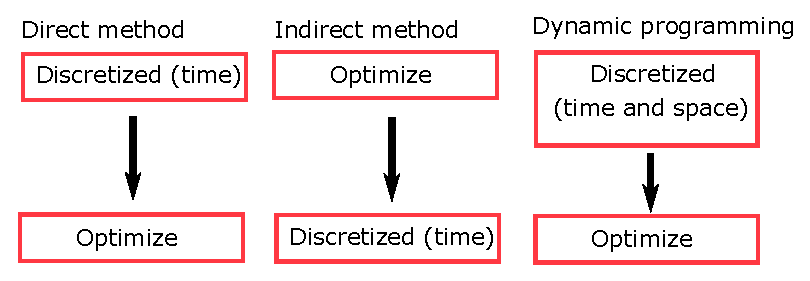
\includegraphics[width=0.8\textwidth]{discretized.eps}
	\caption{Overview of different discretization methods.}
	\label{fig:discretization_m}
\end{figure}

"Since direct methods are best suited to solve practically relevant OCPs" \cite{Mercy2018}, this thesis is following the direct method. To implement the discretization of time when using the Direct method, a time shooting approach is used.

\subsubsection{Time shooting}
A shooting approach makes use of a time grid. Time will be sampled and on every time instant the optimal control problem is assessed. On these discrete points constraints will not violated but there are no limits on the amount of violation between the different time samples. In order to reduce the amount of constraint violation the sampling rate should be taken high enough, while bearing in mind the extra optimization variables introduced and therefore calculation load. An other approach to take constraint violation between different sample points into account, is using spline based optimization formulations. \cite{Mercy2018}\\

Two different shooting approaches exist:\\
\begin{enumerate}
	\item Multiple shooting (MS)\\
	During multiple shooting every new time sample $ns\in \mathbb{N}$ new states and controls are introduced and taken as optimization variables.
	Input changes are only allowed on the different time discrete time instances which leads to a piece wise control input signal. The blue bars indicate in Figure \ref{fig:TS} (left) indicate the control value $U_i$ that is applied to the system.  The red dots are system states that are defined as optimization variables and are not constant during a time interval $\Delta T$. In order to make the connection between states at time $t_i$ and $t_{i+1}$, discrete time integration is used according to $\bm{q}(k+1) = \bm{f}(\bm{q}(k), \bm{u}(k))$. These connections are put as constraints in the discretized optimization formulation of \ref{eq:OCP} and are called in literature 'path closing constraints' \cite{Gillis2019}. \\ Equation \ref{eq:OCP_dis} shows \ref{eq:OCP} when discretized with the multiple shooting approach. 

	\begin{equation}
	\label{eq:OCP_dis}
	\begin{aligned}
	\min_{\bm{q}(.),\bm{u}(.)} \quad & \sum_{k = 0}^{N-1}l_{k}(\bm{q}_{k},\bm{u}_{k}) + E(\bm{q}_{N}) \\
	\textrm{s.t.} \quad & \bm{q}_{k+1} = \bm{f}(\bm{q}_{k}, \bm{u}_{k}) & k = [0,\cdots, N-1]\\
	& \bm{q}_{0}= \bm{q}_{measured} \\
	& \bm{q}_{k}\in Q,\hspace{3 mm} & k = [0,\cdots, N]\\
	& \bm{u}_{k}\in U \hspace{3 mm} & k = [0,\cdots, N-1]\\
	& \bm{q}_{N}\in Q_f,\hspace{3 mm} N \in \mathbb{N}
	\end{aligned}
	\end{equation}
	
	\item Single shooting (SS)\\  
	In the single shooting or sequential approach which is visualized in Figure \ref{fig:TS}(right), only the first state and the controls are taken as optimization variables. Other states during the time horizon are derived from the initial state and the applied control. This is achieved by substituting the states during the control horizon by the integration results from the initial state and the applied controls. The mathematical formulation of this is shown by \ref{eq:2}. In Figure \ref{fig:TS} (right) are the states that result from integration indicated in green. \cite{Gillis2019}
	
	\begin{equation}\label{eq:2}
	\begin{aligned}
	\bm{q}^1 &= \bm{f}(\bm{q}^0, \bm{u}^0)\\
	\bm{q}^2 &= \bm{f}(\bm{f}(\bm{q}^0, \bm{u}^0), \bm{u}^1)\\
	\bm{q}^3 &= \bm{f}(\bm{f}(\bm{f}(\bm{q}^0, \bm{u}^0), \bm{u}^1), \bm{u}^2)\\
	...
	\end{aligned}
	\end{equation}
\end{enumerate}
%\vspace{1 cm}

\begin{figure}[htp]
	\centering
	\begin{minipage}{0.49\textwidth}
		\centering
		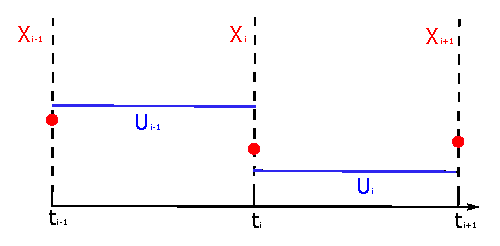
\includegraphics[width=1\textwidth]{MS_int.eps}
	\end{minipage}
	\hfill
	\begin{minipage}{.49\textwidth}
		\centering
		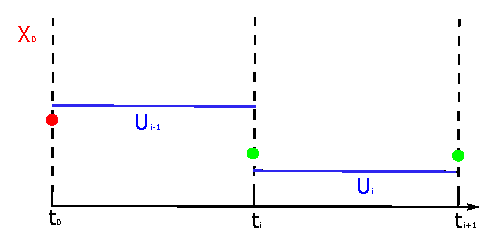
\includegraphics[width=1\textwidth]{SS.eps}
	\end{minipage}
	\caption{Schematic view of the time shooting approaches (left: multiple shooting; right: single shooting).}
	\label{fig:TS}
\end{figure}

In this thesis a multiple shooting approach is used together with the use of a Runge-Kutta integration scheme. Runge-Kutta is an explicit integration scheme which has a higher calculation cost than a standard Euler scheme but is more reliable for non-linear systems and has a higher stability with respect to the chosen time-step. \cite{Mercy2018}  \\ 

The difference between the two shooting approaches is that 'Multiple shooting'(MS) will lead to a larger Hessian of the objective and a larger Jacobian of the constraints. The reason for this is the introduction of more optimization variables. The advantage of MS is then again that these matrices are more sparse because a certain state is only dependent on the previous one and a control input which means they can be used in calculations more efficiently. In single shooting every state depends on the begin state and different controls which gives smaller, more populated matrices which are more calculation expensive. \cite{Gillis2019}

\subsection{Model predictive control}
In slow changing environments as for example a chemical plant, MPC is already a mature approach. More recently this technology also made its introduction in controlling systems with higher dynamics e.g. vehicle control due to an increase of computational power and the use of more efficiently algorithms. \cite{Mercy2018}. In the next section a short introduction of the formulation is made. \\

MPC is an approach were optimizations are solved in a loop in order to be able to notice disturbances, changing environments and model-plant mismatches. Therefore it makes use of a moving time horizon\footnote{There are also other implementations e.g. shrinking time horizon, where the prediction time gets smaller every step.}. Every iteration an OCP is solved over the prediction horizon and as result control signals are given as output. Only the first control is applied for one time interval of the finite prediction horizon $N\cdot T_{s}$ as is visualized in Figures \ref{fig:MPC1}and \ref{fig:MPC2}.

The decision on the amount of samples $N$ that are used in the control horizon is based on a trade off between higher accuracy and calculation effort. \cite{TongDuySon2019, Mercy2018}. In Figure \ref{fig:MPC1} the solving of an OCP during one MPC iteration on time sample $t+1$ is depicted. Figure \ref{fig:MPC2} shows than only the first control of the obtained control signal will be applied, which induces the system to come in a different state which will be the new start state and a new OCP will be solved. This will go on until the final desired conditions are met. A single OCP iteration only takes the model of the system into account as is done in a feedforward controller but over the iterations a feedback loop is acquired because of the changing initial state \cite{Patrinos2019}\\

\begin{figure}[h!]
	\centering
	\includegraphics[width=0.6\textwidth]{MPC1.PNG}
	\caption{Visualization of the optimal control problem solved in one iteration of the MPC (Source: \cite{Patrinos2019}).}
	\label{fig:MPC1}
\end{figure}

\begin{figure}[h!]
	\centering
	\includegraphics[width=0.6\textwidth]{MPC2.PNG}
	\caption{Visualization of the application of the first step of the calculated control signal during one iteration of the MPC (Source:\cite{Patrinos2019}).}
	\label{fig:MPC2}
\end{figure}

\newpage





%\begin{equation}\label{eq:3}
%minimize_{\bm{q}(.),\bm{u}(.)}\sum_{k = 0}^{N-1}l_{k}(\bm{q}_{k},\bm{u}_{k}) + E(\bm{q}_{N})
%\end{equation}
%\hspace{42 mm} \textit{subject to:}
%\[\bm{\dot{q}}_{k+1} = \sum_{k = 0}^{N-1}\bm{f}(\bm{q}_{k}, \bm{u}_{k})\]
%\[\bm{q}_{0}= \bm{q}_{measured}\]
%\[h(\bm{q}_{k},\bm{u}_{k}) \geq 0\]
%\[\bm{q}_{k}\in Q,\hspace{3 mm} \bm{u}_{k}\in U, \hspace{3 mm} N \in \mathbb{N}\]


Equation \ref{eq:MPC} is a representation of the solved discrete system OCP during one iteration of the MPC. It is a discretized version of equation \ref{eq:OCP}. The Runge-Kutta integration is embedded in $\bm{f}$. The hard constraints are represented by $h$. It is worth noticing that the constraints can be violated in-between the different time sample points.\\ \cite{Panos_opti}

MPC has no direct feedback loop, but through the iterative way of solving the OCPs it can still deal with model mismatch or a changing environment. The downside of this approach is that it requires a bigger computational load, which makes efficiently written software a necessity. 


%%% Local Variables: 
%%% mode: latex
%%% TeX-master: "thesis"
%%% End: 
\chapter{Learning from ideal data\\}
\label{cha:Learning_algorithm}

This chapter is focussing on the implementation of the inverse reinforcement learning idea that is explained at the end of chapter \ref{cha:Literature_study}. It will start with a detailed explanation and discussion of the simulations done in order to check what the algorithm is capable of. In this chapter an ideal situation is assumed which means that data is generated with the same vehicle model used to learn the weights and the assumption that the observations are generated as the solutions of a cost function similar to \ref{eq:1} is exactly fulfilled. Afterwards the step is made to use a more sophisticated 15 degrees of freedom vehicle model with the use of the Amesim software and it is checked how accurate results are learned when the assumption on the observations is violated. Next a new learning approach is proposed which is based on a fitting algorithm and makes use of taylor expansions. 

\section{Ideal learning situation }

\textbf{Deze sectie moet nog herschreven worden en nagekeken}

\subsection{Non-linear vehicle model}\label{sec:Vehicle_models}
In this paper the controller is designed on top of a nonlinear bicycle model \cite{TongDuySon2019} as can be seen in figure \ref{fig:bicycle_model}.\\

\begin{figure}[h!]
	\centering
	\includegraphics[width=0.5\textwidth]{Bicycle_model_paper.png}
	\caption{Non-linear vehicle bicycle model (Source: \cite{TongDuySon2019}).}
	\label{fig:bicycle_model}
\end{figure}

In this model, the vehicle system is characterised with 6 states and 2 inputs:
\begin{equation}\label{eq:bicycle_model}
\centering
\bm{x} = 
\begin{bmatrix}
X & Y & v_x & v_y & \psi & \dot{\psi}
\end{bmatrix}^{T}
\; and \; \bm{u} = 
\begin{bmatrix}
t_r & \delta
\end{bmatrix}^{T}
\end{equation}

In this formulation, $X$ and $Y$ are the position of the centre of the car in the global coordinate system (capital symbols). $\psi$ is the vehicle yaw angle and $\dot{\psi}$ the yaw angular velocity. $v_x$ and $v_y$ are the vehicle velocities in the local vehicle frame (small symbols). The input vector consists of the throttle control input $t_r$ and the steering angle $\delta$.\\

The equations of motion \cite{TongDuySon2019} are:
\begin{equation}\label{eq:bicycle_model_eqmotion}
\begin{aligned}
\dot{X} = v_x cos(\psi) - v_y sin(\psi)\\
\dot{Y} = v_x sin(\psi) + v_y cos(\psi)\\
\dot{\psi} = \dot{\psi}\\
m \dot{v}_x = F_{x,f} cos(\delta) - F_{y,f} sin(\delta) + F_{x,r} - F_{drag} + m v_y \dot{\psi}\\
m \dot{v}_y = F_{x,f} sin(\delta) + F_{y,f} cos(\delta) + F_{y,r} - m v_x \dot{\psi}\\
I_z \ddot{\psi} = L_f (F_{y,f} cos(\delta) + F_{x,f} sin(\delta)) - L_r F_{y,r}
\end{aligned}
\end{equation}

The used fixed parameters are the total vehicle mass $m$, the z-axis moment of inertia $I_z$ and the distances between the centre of gravity (COG) and the front and rear axle $L_f$ and $L_r$.\\

The drag force is calculated as:
\begin{equation}\label{eq:bicycle_Fdrag}
\begin{aligned}
F_{drag} = C_{r0} + C_{r1} v_x^2
\end{aligned}
\end{equation},
with $C_{r0}$ the roll resistance and $C_{r1}$ the air drag contributions.\\

To calculate the tyre forces, a linear tyre model is used. The longitudinal tyre forces are calculated as:
\begin{equation}\label{eq:bicycle_Fx}
\begin{aligned}
F_{x,f} = \frac{t_r T_{max}}{2 R_w}\\
F_{x,r} = F_{x, f}
\end{aligned}
\end{equation}

$R_w$ is the wheel radius and $T_{max}$ a measure for the maximum torque the engine is able to supply. In this way, four wheel drive is assumed and the total torque is equally distributed between front and rear axle (division by 2 in above equations). The coefficient $t_r$ is the normalised wheel torque and can have a value between -1 and 1 (negative for braking).
The lateral tyre forces are calculated based on the tyre slipangles $\alpha_f$ and $\alpha_r$:
\begin{equation}\label{eq:bicycle_slipangle}
\begin{aligned}
\alpha_f = -atan(\frac{\dot{\psi} L_f + v_y}{v_x}) + \delta\\
\alpha_r = atan(\frac{\dot{\psi} L_r - v_y}{v_x})
\end{aligned}
\end{equation},
resulting in:
\begin{equation}\label{eq:bicycle_Fy}
\begin{aligned}
F_{y,f} = 2 K_f \alpha_f\\
F_{y,r} = 2 K_r \alpha_r
\end{aligned}
\end{equation}\\
The use of this linearised lateral tyre model is valid for small lateral accelerations ($a_y <= 4 m/s^2$) and slip angles ($\alpha <= 5^o$) \cite{TongDuySon2019}. It is acceptable to use this model in this paper as the goal is to control a comfortable and thus smooth lane change manoeuvre. These constraints will also be checked during the validation.\\

The fixed model parameter used during the simulations are given in table \ref{table:vehicel_model_param}. These correspond to common used vehicle parameters as found in paper \cite{Yankov}.

\begin{table}[h]
	\centering
	\begin{tabular}{|p{5cm}|p{2cm}|}
		\hline
		\textbf{Parameter} & \textbf{Value}\\ \hline		
		Vehicle mass $m$ [kg] & 1430\\ \hline
		Moment of inertia $I_z$ [$kgm^2$] & 1300\\ \hline
		Front axle distance $L_f$ [m] & 1.056\\ \hline
		Rear axle distance $L_r$ [m] & 1.344\\ \hline
		Roll resistance coefficient $C_{r0}$ [N] & 0.6\\ \hline
		Air drag coefficient $C_{r1}$ [$\frac{Ns^2}{m^2}$] & 0.1\\ \hline
		Engine torque limit $T_{max}$ [Nm] & 584\\ \hline
		Wheel radius $R_w$ [m] & 0.292\\ \hline
		Lateral front tyre stiffness $K_{f}$ [N] & 41850.85\\ \hline
		Lateral rear tyre stiffness $K_{r}$ [N] & 51175.78\\ \hline
		
	\end{tabular}
	\caption{Used vehicle model parameters.}
	\label{table:vehicel_model_param}
\end{table}

\subsection{defining the problem}
\textbf{Kijk slides 31 maart na, problem definition helemaal op het einde nog verwerken in de tekst.}

The method applied in order to check the consistency of the learning algorithm is to generate data that are generated by solving the 











%Bespreek het vehicle model. Lees featueres stukje na dat geschreven heb voor taak VS. X en Y variables zijn in longitudinal axis. Maakt gebruik van een complexer model --> kromming van het pad zit al inherent in de normal acceleration van het voertuig. --> versnellingen die ik beschouw zijn de totale versnellingen. 
%
%%An overview of the flow of the algorithm can be seen in Figure blablabla. (Explain flow of code and make connections with the above explained theory behind the model.)
%
%De gevonden trajectories vergelijken met een standaard lane change uit de literatuur --> zie $lane_change_kin$ voor foto. \\
%
%Zeg dat eerst de appraoch was tested in ideale omstandigheden: zelfde voertuigmodel werd gebruikt en de assumptie dat de date is gegenereerd door de minimalizatie van een comfort kostfunctie werd aan voldaan. 
%
%
%Herinner de lezer nog even de structuur die gaat worden gevolgd. 
%Learning, planning, tracking, validatie.
%Dit hoofdstuk zal over de learning gaan.
%Hoe is algorithm opgebouwd? Wrm wordt dit zo gedaan?
%Welke vehicle modellen wordt er gebruikt? Wrm mag men hier een simple vehicle mode gebruiken?
%Dit is gemachtigd omdat men hier de omgeving wil scannen voor een feasible pad --> dit wordt trager gedaan dan de tracking.(tracking zal gebruik maken van een meer complex model) Path planning ligt focus vooral op de omgeving.
%Goed refereren naar het rapport en VS rapport
%Wat zijn de assumpties die werden genomen?
%
%Hoe zal de methode gevalideerd worden? Leg de twee methodes uit: code generatie en kijken of de wegings factoren terug gevonden kunnen worden? Mappen de feature values met de values van het geobserveerde pad? --> is het doel dat gevolgd probeert te worden haalbaar? 
%
%Ga hier niet meer te diep in op de entropie. Leg het hier meer intuitief uit om de lezer niet te verwaren. 
%
%Vermeld afleiding van algortihm. Leg uit in Thesis hoe komt aan gradient die gebruikt. Zie papers: Ziebart et al and Kretzschmar et al.
%
%Modeleer een andere bestuurder. Can try to reproduce a data set with a change of parameters which represents a different driver. Can check that the learned model is also different. Hiermee aantonen dat er ook echt andere wegingsfactoren worden gegenereerd en dat de specifieke driving characteristics worden meegenomen.
%
%Ligt een tipje van de sluier op : hoe zal de data gegenereerd worden? 
%Plot simulink model en duidt de blokken aan die zullen worden ingevuld. Hier gaat dieper in gegaan worden in de volgende hoofdstukken. 
%
%Maak een vermelding dat men het menselijke gedrag van het geleerde model kan nagaan met een Turing test.\\
%
%Maak een plotje zoals paper Learning to Predict Trajectories of Cooperatively Navigating Agents --> feature variance afwijking en average error. (zelfde plotjes als al de papers)\\
%
%Schrijf een paragraaf over hoe de data gegenereerd wordt. --> leg kort het gebruik van de verschillende vehicle modellen uit. 
%
%
%
%Schrijf een paragraaf over de theta update --> zie RPROP methode --> beschrijf wrm beter is dan andere methodes die gezien werden. Bespreek hoe de parameters werden gekozen. 
%
%
%Kan vermelding maken dat in deze thesis de features zijn gekozen met de hand --> men kan proberen om de features ook te leren van date (Characterizing Driving Styles with Deep Learning)
%
%\clearpage
%
%
%%Afleiding van exponentiël functie zie paper: Feature-based prediction of trajectories for socially compliant navigation (foto) --> weights are lagrange coefficients.


%\section{Tables}
%Tables are used to present data neatly arranged. A table is normally
%not a spreadsheet! Compare \tref{tab:wrong} en \tref{tab:ok}: which table do
%you prefer?
%
%\begin{table}
%  \centering
%  \begin{tabular}{||l|lr||} \hline
%    gnats     & gram      & \$13.65 \\ \cline{2-3}
%              & each      & .01 \\ \hline
%    gnu       & stuffed   & 92.50 \\ \cline{1-1} \cline{3-3}
%    emu       &           & 33.33 \\ \hline
%    armadillo & frozen    & 8.99 \\ \hline
%  \end{tabular}
%  \caption{A table with the wrong layout.}
%  \label{tab:wrong}
%\end{table}
%
%\begin{table}
%  \centering
%  \begin{tabular}{@{}llr@{}} \toprule
%    \multicolumn{2}{c}{Item} \\ \cmidrule(r){1-2}
%    Animal    & Description & Price (\$)\\ \midrule
%    Gnat      & per gram    & 13.65 \\
%              & each        & 0.01 \\
%    Gnu       & stuffed     & 92.50 \\
%    Emu       & stuffed     & 33.33 \\
%    Armadillo & frozen      & 8.99 \\ \bottomrule
%  \end{tabular}
%  \caption{A table with the correct layout.}
%  \label{tab:ok}
%\end{table}




%%% Local Variables: 
%%% mode: latex
%%% TeX-master: "thesis"
%%% End: 

\chapter{Learning from ideal data}
\label{cha:Learning_algorithm}
This chapter focusses on implementing the learning of the different weighting factors in the comfort cost function $\bm{\theta}^T\bm{F}(\bm{r})$, following the methods explained in \ref{s:inverse re le}. The use of ideal data is assumed which means that vehicle model mismatch is avoided by using the same model for learning the weighting factors and generating data. Thereby is the approximation that comfort of a driver is modelled by a linear relation of features, exactly fulfilled. Data is generated by choosing a set of weighting factors in order to produce kinematic vehicle signals by minimizing Eq. (\ref{eq:6a}). A validation of the developed learning algorithm is done when the chosen weighting factors used in generating the data are retrieved.\\

First, the non-linear bicycle model and the used parameters are explained in section \ref{sec:Vehicle_models}. A non-linear bicycle model has been chosen because this can sufficiently model the dynamics during a comfortable lane change maneuver and the calculation cost stays affordable. The model makes abstraction of suspension dynamics i.e. neglects rolling and pitching and the position of the centre of gravity is fixed on the vehicle during driving \cite{Yankov}. Further on, the developed algorithm to learn the weight from demonstration is discussed in section \ref{s:learning_alg}. Afterwards it is shown how the ideal data is generated and validated in section \ref{s:GD} and the learning results are analysed in section \ref{s:ID_results}.\\
As noted before the learning process discussed, concerns an offline optimization which allows for higher calculation loads because of the absence of pushing real time constraints.

\begin{figure}[h!]
	\centering
	\includegraphics[width=0.5\textwidth]{Bicycle_model_paper.png}
	\caption{Non-linear bicycle model (Source: \cite{TongDuySon2019}).}
	\label{fig:bicycle_model}
\end{figure}

\section{Non-linear bicycle model}\label{sec:Vehicle_models}
The free body diagram of the non-linear bicycle model can be seen in figure \ref{fig:bicycle_model}.

Two variants of this model are discussed which are differentiated by the smoothness of the controls that are used. 
\begin{enumerate}
	\item	Model has 6 states and 2 controls: 
	\begin{equation}\label{eq:bicycle_model1}
	\centering
	\bm{X} = 
	\begin{bmatrix}
	x & y & v_x & v_y & \psi & \dot{\psi}
	\end{bmatrix}^{T}
	\; and \hspace{2mm} \; \bm{U} = 
	\begin{bmatrix}
	t_r & \delta
	\end{bmatrix}^{T}.
	\end{equation}
	
	\item Model has 10 states and 2 controls:
	\begin{equation}\label{eq:bicycle_model2}
	\centering
	\bm{X} = 
	\begin{bmatrix}
	x & y & v_x & v_y & \psi & \dot{\psi} & t_r & \delta & a_x & a_y
	\end{bmatrix}^{T}
	\; and \hspace{2mm} \; \bm{U} = 
	\begin{bmatrix}
	\dot{t_r} & \dot{\delta}
	\end{bmatrix}^{T}.
	\end{equation}
\end{enumerate}


$x$ and $y$ in the above formulation are the position of the centre of gravity of the vehicle in the global coordinate system. $v_x$ and $v_y$ are the vehicle velocities in the local vehicle frame. $\psi$ is the vehicle yaw angle and $\dot{\psi}$ the yaw rate. The control vector of Eq. (\ref{eq:bicycle_model1}) consists of the throttle $t_r$ and the angle of the front wheel $\delta$. In the more extended bicycle model Eq. (\ref{eq:bicycle_model2}), throttle and front wheel angle serve as states. $a_x$ and $a_y$ are the total accelerations of the centre of gravity in the local vehicle frame. The inputs in this second formulation are the first order derivatives of throttle and front wheel angle.\\

The equations of motion derived and checked in literature \cite{TongDuySon2019} are\footnote{Appendix \ref{app:A} shows the complete jerk equations $j_x$ and $j_y$.} :
\begin{equation}\label{eq:bicycle_model_eqmotion}
\begin{aligned}
\dot{x} = v_x cos(\psi) - v_y sin(\psi),\\
\dot{y} = v_x sin(\psi) + v_y cos(\psi),\\
m \dot{v}_x = F_{x,f} cos(\delta) - F_{y,f} sin(\delta) + F_{x,r} - F_{drag} + m v_y \dot{\psi},\\
m \dot{v}_y = F_{x,f} sin(\delta) + F_{y,f} cos(\delta) + F_{y,r} - m v_x \dot{\psi},\\
\dot{\psi} = \dot{\psi},\\
I_z \ddot{\psi} = L_f (F_{y,f} cos(\delta) + F_{x,f} sin(\delta)) - L_r F_{y,r},\\
\dot{t_r} = \dot{t_r},\\
\dot{\delta} = \dot{\delta},\\
a_{tx} = \dot{v}_x,\\
a_{nx} = -v_y\dot{\psi},\\
a_{ty} = \dot{v}_y,\\
a_{ny} = v_x\dot{\psi},\\
j_x = \dot{a}_{tx} + \dot{a}_{nx},\\
j_y = \dot{a}_{ty} + \dot{a}_{ny}  .
\end{aligned}
\end{equation}
\newpage
The drag force is calculated as:
\begin{equation}\label{eq:bicycle_Fdrag}
\begin{aligned}
F_{drag} = C_{r0} + C_{r1} v_x^2
\end{aligned},
\end{equation}
with $C_{r0}$ the roll resistance and $C_{r1}$ the air drag contributions.\\

To calculate the tyre forces, a linear tyre model is used instead of a more complex non-linear model e.g. Pacejka tyre model. The longitudinal tyre forces are calculated as:
\begin{equation}\label{eq:bicycle_Fx}
\begin{aligned}
F_{x,f} = \frac{t_r T_{max}}{2 R_w},\\
F_{x,r} = F_{x, f}.
\end{aligned}
\end{equation}

$R_w$ is the wheel radius and $T_{max}$ the maximum torque the engine is able to supply. Because $F_{x,r} = F_{x, f}$ the longitudinal forces that are induced by the engine are equally distributed between front and rear axle (division by 2 in above equations). The coefficient $t_r$ is the normalised amount of throttle that can be applied and has a value between -1 and 1 (negative for braking). In the bicycle model it is assumed that braking behaves the same as giving a negative amount of throttle.
The lateral tyre forces are calculated based on the tyre slip angles $\alpha_f$ and $\alpha_r$:
\begin{equation}\label{eq:bicycle_slipangle}
\begin{aligned}
\alpha_f = -atan(\frac{\dot{\psi} L_f + v_y}{v_x}) + \delta,\\
\alpha_r = atan(\frac{\dot{\psi} L_r - v_y}{v_x}),
\end{aligned}
\end{equation}
resulting in:
\begin{equation}\label{eq:bicycle_Fy}
\begin{aligned}
F_{y,f} = 2 K_f \alpha_f,\\
F_{y,r} = 2 K_r \alpha_r.
\end{aligned}
\end{equation}\\
The use of this linearised lateral tyre model is valid for small lateral accelerations ($a_y <= 4 m/s^2$) and slip angles ($\alpha <= 5^o$) \cite{TongDuySon2019}. It is acceptable to use this approximate model in this thesis as the goal is to learn a comfortable and thus smooth lane change manoeuvre. However, these constraints will be checked during section \ref{s:GD_val}.\\

The vehicle model parameters used are described in table \ref{table:vehicel_model_param}. These values were provided by Siemens Digital Industries Software. The $Gsteerfactor$ is used to approximate the relation between the front wheel angle and the steer wheel angle turned by the driver, linearly according to: $\delta = \frac{\delta_s}{Gs}$.  

\begin{table}[h]
	\centering
	\begin{tabular}{|p{5cm}|p{2cm}|}
		\hline
		\textbf{Parameter} & \textbf{Value}\\ \hline	
		Vehicle mass $m$ [kg] & 1430\\ \hline
		Moment of inertia $I_z$ [$kgm^2$] & 1300\\ \hline
		Front axle distance $L_f$ [m] & 1.056\\ \hline
		Rear axle distance $L_r$ [m] & 1.344\\ \hline
		Roll resistance coefficient $C_{r0}$ [N] & 0.6\\ \hline
		Air drag coefficient $C_{r1}$ [$\frac{Ns^2}{m^2}$] & 0.1\\ \hline
		Engine torque limit $T_{max}$ [Nm] & 584\\ \hline
		Wheel radius $R_w$ [m] & 0.292\\ \hline
		Lateral front tyre stiffness $K_{f}$ [N] & 41850.85\\ \hline
		Lateral rear tyre stiffness $K_{r}$ [N] & 51175.78\\ \hline
		Gsteerfactor $Gs$ [-] &16.96 \\ \hline
		
	\end{tabular}
	\caption{Used vehicle model parameters.}
	\label{table:vehicel_model_param}
\end{table}
\newpage
\section{Learning algorithm} 
\label{s:learning_alg}
The goal of the learning algorithm is to learn the weighting factors $\bm{\theta}$ in the comfort objective function: $\bm{\theta}^T\bm{F}(\bm{r})$. Its formulation is presented in section \ref{s:flow alg}. The features that are the entries of the feature vector $\bm{F}(\bm{r})$ capture a notion of comfort felt by the driver. Based on the literature study displayed in Chapter \ref{cha:Literature_study} and on paper \cite{Kuderer2015a}, the comfort criteria embedded in the different feature values are presented in section \ref{s:obj}. The scenario of a lane change on a straight road is modelled with the time horizon of the maneuver itself taken as an optimization variable $T$.


\subsection{Formulation of the algorithm}\label{s:flow alg}
%The goal of the learning algorithm is to output weighting factors that when applied in the objective $\bm{\theta}^T\bm{F}(\bm{r})$, generate feature vector  $\bm{F(\bm{r})}$ that are the best possible fit with the observed feature vector. Without a vehicle mismatch a match of feature values will directly induce a good match of the kinematic signals as is extensively discussed in section \ref{s:ID_results}. 

%This means that similarity between the observed path and the one that follows from minimizing the objective $\bm{\theta}^T\bm{F}(\bm{r})$ for chosen weighting factors, is quantified by the difference between the feature values of the observed path and the obtained one. 

As has been discussed in chapter \ref{cha:Literature_study},  $\bm{\theta}_{opti}$ gives the best possible fit between $\bm{F}(\bm{r}_{expected})$ and $\bm{F_{obs}(\bm{r}_{obs})}$.
Without vehicle mismatch, a match of feature values will induce a good match of the kinematic vehicle signals as will be further discussed in section \ref{s:ID_results}.
The flow of a single dataset learning algorithm can be seen in Figure \ref{fig:basic learning}.\\

%The path that is expected to be produced by the driver is the path that is felt as the most comfortable and equals $\bm{r}_{expected} =  \underset{\bm{r}}{\argmin} \hspace{1mm}  \bm{\theta}^T\cdot \bm{F}(\bm{r})$.\\

The learning is started by proposing a set of weighting factors e.g. all equal to one. Eq. (\ref{eq:6a})  is minimized in order to generate an expected path. From this $\bm{F}(\bm{r}_{expected})$ can be retrieved by using the definition discussed in section \ref{s:obj}. Afterwards, the relative features $f_{rel,i}$ are calculated by element-wise  divide  the expected feature vector by the observed one $\bm{F}_{obs}$. A perfect match is acquired when the division equals one and the learning algorithm is terminated. The tolerance on convergence towards one, is chosen during this chapter equal to $10^{-3}$.\\
\vspace{5mm}

\begin{figure}[h!]
	\centering
	\includegraphics[width=1.0\textwidth]{basic_learning.png}
	\caption{Basic flow of the inverse optimal control algorithm.}
	\label{fig:basic learning}
\end{figure}

  
While no convergence takes place the weighting factors are updated, making use of the estimation of the approximated gradient and the RPROP algorithm explained in Chapter \ref{cha:Literature_study}. The new weighting factors are used to calculate a new expected path which will result in different expected feature values $\bm{F}(\bm{r}_{expected})$.  Next, a more detailed description of the calculation of the expected path is given by Eq. (\ref{opt:basic_opti_w}) which uses as vehicle model Eq. (\ref{eq:bicycle_model2}). \\

%In order to apply the RPROP method only the sign of the gradient is used which means that the size of the gradient is decoupled from the update value of the weighting factors. The estimate of the gradient is given by $\pdv{\bm{F}}{\bm{\theta}} = \bm{F}_{obs} - \bm{F}(\bm{r}_{expected})$  and the update of the weight is achieved by applying the gradient method according to $\bm{\theta}^{k+1} = \bm{\theta}^{k} - |\Delta \theta^{k}|sign( \pdv{\bm{F}}{\bm{\theta}}^k )$ where $\Delta \theta^{k}$ is calculated according section \ref{s:RPROP}. If follows that the weight $\theta_i$ is decreased if $f_{obs,i}>f_{i}(\bm{r_{exptected}})$ and increased when $f_{obs,i}<f_{i}(\bm{r}_{exptected})$.

\begin{equation}\label{opt:basic_opti_w}
\begin{aligned}
\min_{\bm{X}(.),\bm{U}(.), T} \quad &  \bm{\theta}^T\bm{F}(\bm{X},\bm{U}, T) \\
\textrm{s.t.} \quad & \bm{X}^{k+1} = I(\bm{X}^{k}, \bm{U}^{k}) & k = [0,\cdots, N-1]\\
& \bm{X}^{0}[1:8]= \bm{X}_{intitial} \\
& T \leq T_{limit}\\
& \bm{F}(\bm{X}^{k}) \geq 0	& k = [0,\cdots, N]\\
& \bm{H}(\bm{X}^{k}) = 0	& k = [0,\cdots, N]\\
& \bm{X}^{k}\in \mathbb{R}^{10\times 1}  & k = [0,\cdots, N]\\
& \bm{U}^{k}\in \mathbb{R}^{2\times 1} \hspace{3 mm} & k = [0,\cdots, N-1]\\
& T \in \mathbb{R},\hspace{3 mm} N \in \mathbb{N}
\end{aligned}
\end{equation}

Where $\bm{X} \in \mathbb{R}^{10\times N+1}$ and $\bm{U}\in \mathbb{R}^{2\times N}$ contain respectively the states and controls of Eq.(\ref{eq:bicycle_model2}) during the maneuver. The time of the maneuver is represented as $T$. In order to discretize time, a multiple shooting approach is adopted as explained in section \ref{s:time_dis}. The amount of integration intervals $N$ is chosen equal to $1000$ and determines the  amount of controls applied to go from the initial state towards the end state. 
Inside the function $I$ the Runge-Kutta time integration method is embedded in order to connect different states when a certain control is applied for $\Delta T$. Here the equations of motion Eq. (\ref{eq:bicycle_model_eqmotion}) are inputted in the optimization because derivatives of the vehicle states are needed. The time discretization used can be categorized as a direct method and because a multiple shooting approach is conducted at every time instance, a new set of state optimization variables is introduced. The path constraint vector $\bm{F}$ demarcates together with the equality constraint vector $\bm{H}$, the feasible space of the solutions for $\bm{X}$ and $\bm{U}$. An overview of the constraints used, is given by Eq. (\ref{eq:F}) and Eq. (\ref{eq:H})

\begin{equation}\label{eq:F}
\bm{F} =
\begin{Bmatrix}
-\frac{Width\hspace{1mm}Lane}{2} \leq y^k \leq \frac{3\cdot Width\hspace{1mm}Lane}{2}, & k = [0,\cdots, N] \\
0 \leq x^k, & k = [0,\cdots, N] \\
-\frac{\pi\cdot 150}{180 Gs} \leq \delta^k \leq \frac{\pi\cdot 150}{180 Gs}, & k = [0,\cdots, N] \\
-1 \leq t_r^k \leq 1, & k = [0,\cdots, N]

\end{Bmatrix},
\end{equation}\\

\begin{equation}\label{eq:H}
\bm{H} =
\begin{Bmatrix}
y^N = Width\hspace{1mm}Lane \\ \vspace{1mm}
vy^N = 0 \\\vspace{1mm}
\psi^N = 0 \\\vspace{1mm}
\dot{\psi}^N = 0 \\\vspace{1mm}
\delta^N = 0 

\end{Bmatrix}.
\end{equation}\vspace{5mm}

The constraints displayed in $\bm{H}$ make sure that at the end of the lane change, the slip angles in the tires and the steer wheel angle are zero. From Eq. (\ref{eq:bicycle_model_eqmotion}) this induces that the lateral velocity, acceleration and yaw acceleration also become zero and this marks the end of the lane change. $y^N$ ensures that the wanted lateral distance is covered. This distance can be calculated from the start position of the vehicle and the width of the lane in order to end up at the centre line of the desired lane. \\ At the start of the lane change, straight driving at constant longitudinal speed is assumed. To achieve this, the constraints of Eq. (\ref{eq:X0}) are used. No constraints for acceleration is needed. This would give a redundancy due to the other initial states in combination with the equations of motion \ref{eq:bicycle_model_eqmotion}. In Eq. (\ref{eq:X0}) all initial states are zero except the initial speed $v_{x,start}$ and $t_{r,start}$. The amount of throttle at the start of the lane change is chosen to overcome the aerodynamic drag without accelerating. This is given by $t_r^0 = \frac{(C_{r0}+C_{r1}v_{start}^2)r_w}{T_{max}}$. Therefore, it can be concluded that the parameters that distinguish different lane changes are $v_{x,start}$ and $Width\hspace{1mm}Lane$. This is exploited when generating different ideal lane change datasets for chosen weighting factors. 
\newpage
\begin{equation}\label{eq:X0}
\bm{X}_{initial} =
\begin{bmatrix}
 x_{start}\\ 
 y_{start}\\
 v_{x,start}\\
 v_{y,start}\\
 \psi_{start}\\
 \dot{\psi}_{start}\\
 t_{r,start}\\
 \delta_{start}\\

\end{bmatrix}
\end{equation}


% discuss time limit is chosen equal to 25 s.
The time limit constraint in Eq. (\ref{opt:basic_opti_w}) is needed in order to demarcate the optimization solution space. When set, it has to take two conflicting criteria into account. It has to be chosen large enough in order to have a minor influence on the lane change behaviour introduced by this constraint. Secondly, it has to be taken small enough to preserve good conditions for the numerical integration performed inside $\bm{F}(\bm{X},\bm{U}, T)$, as will be seen in in \ref{s:obj}. This is because the number of optimization points $N+1$ of the states is fixed, which means that a larger time limit will give a coarser time discretization. In this thesis the time limits used are $25\hspace{1mm}s$ and $30\hspace{1mm}s$, which is a compromise between the two criteria. This choice is validated in section \ref{s:GD_val}.\\It is worth noting that with the removal of the time limit constraint the optimized comfortable lane change takes around $160 \hspace{1mm}s$. This is not a realistic results because the objective will, as previously explained, not have good numerical properties.\\ 

In order to solve Eq. (\ref{opt:basic_opti_w}) an initial guess is needed for the longitudinal velocity in order to avoid the emergence of an invalid number. The default initial guess used in the CasADi software is an all zero vector. As can be seen in Eq. (\ref{eq:bicycle_slipangle}) this would give a division by zero in the calculation of the slip angles. \\
To further enhance the solving speed of Eq. (\ref{opt:basic_opti_w}) also initial guesses are given for the other vehicle states and additionally the controls. To do this, a feasible solution of the non-linear bicycle model for a lane change is needed because IPOPT is an interior point method. Therefore, the initial guesses for $\bm{X}, \bm{U} \;and\; T$ are taken from the observed ideal data. \\

Another way to speed up the solving time of the IPOPT solver, is setting the initial guess of the lambda multipliers internally used, equal to the ones found during the previous call of Eq. (\ref{opt:basic_opti_w}) during the loop visualized by figure \ref{fig:basic learning}. \\The time needed for the CPU to calculate the expected path for a certain set of weighting factors and thus solving Eq. (\ref{opt:basic_opti_w}), takes around $5\hspace{1mm}s$ (python implementation) when a time limit of $30$ seconds and N equal to $1000$ is chosen.\\

As discussed above, the solver used to calculate the states and control signals in Eq. (\ref{opt:basic_opti_w}), is IPOPT which is an open source solver. The idea behind it is to smoothing the KKT conditions and transform it into a smooth root finding problem. \cite{Panos_opti} \\

%Because IPOPT is a interior boundary method, a feasible initial guess is needed.
% Every time that the expected path has to be calculated as is visualised in flow diagram \ref{fig:basic learning}, the optimization \ref{opt:basic_opti_w} is performed with as initial guess the observed maneuver.\\

\subsection{Objective function}\label{s:obj}
The objective function used in Eq. (\ref{opt:basic_opti_w}) has to represent comfort felt by the driver and is based on the literature study displayed in section \ref{s:comfort_parameters}. The choice made in how to define the different features is important because it sets the fixed framework where the weighting factors will be learned in. It can be expected that the linear relation of features given by $\bm{\theta}^T\bm{F}(\bm{r})$ will serve as an approximation for the real, more complex comfort objective of a human drive. The feature framework that is further discussed in this section, can be validated and adjusted based on an user study.\\

%As is shown in \cite this linear approximation of features can already capture  the main trends that contribute to an comfortable maneuver experience.

\begin{equation}\label{eq:obj}
discomfort = \theta_1 \cdot f_1 +\theta_2 \cdot f_2 +\theta_3 \cdot f_3 +\theta_4 \cdot f_4 +\theta_5 \cdot f_5 +\theta_6 \cdot f_6 \\
\end{equation}
\[	f_i, \theta_i \in \mathbb{R} \hspace{5mm}
i \in \mathbb{N}\]


\textit{Feature 1: longitudinal acceleration}
\begin{equation}\label{eq:flong_acc}
f_{1}:\bm{r}\xrightarrow{}f_1(\bm{r})=\int_{0}^{T}a_{x,total}^{2}(t) dt
\end{equation}
Feature one assesses the amount of discomfort by integrating the total longitudinal acceleration in the local axis. The local axis is fixed to the centre of gravity of the vehicle, as can be seen in Figure \ref{fig:bicycle_model}. The total longitudinal acceleration  $a_{x,total} $ is the sum of  $ a_{x,tangential}$ and $a_{x,normal}$ as described in Eq. (\ref{eq:bicycle_model_eqmotion}). \\

\textit{Feature 2: lateral acceleration}
\begin{equation}\label{eq:flat_acc}
f_{2}:\bm{r}\xrightarrow{}f_2(\bm{r})=\int_{0}^{T}a_{y,total}^{2}(t) dt
\end{equation}
Feature two assesses the amount of discomfort by integrating the total lateral acceleration in the local axis. The total lateral acceleration  $a_{y,total} $ is the sum of  $ a_{x,tangential}$ and $a_{x,normal}$ as described in Eq. (\ref{eq:bicycle_model_eqmotion}).\\

\textit{Feature 3: longitudinal jerk}
\begin{equation}\label{eq:flong_jerk}
f_{3}:\bm{r}\xrightarrow{}f_3(\bm{r})=\int_{0}^{T}j_{x}^{2}(t) dt
\end{equation}
Feature three gives the amount of comfort by integrating the total change of longitudinal acceleration during the followed path. \\

\textit{Feature 4: lateral jerk}
\begin{equation}\label{eq:flat_jerk}
f_{4}:\bm{r}\xrightarrow{}f_4(\bm{r})=\int_{0}^{T}j_y^{2}(t) dt
\end{equation}
Feature four gives the amount of comfort by integrating the total change of lateral acceleration during the followed path. \\

\textit{Feature 5: desired speed}
\begin{equation}\label{eq:des_speed}
f_{5}:\bm{r}\xrightarrow{}f_5(\bm{r})=\int_{0}^{T}(v_{des}-v_x)^2 dt
\end{equation}
$v_{des}$ is assumed to be a constant value and set equal to the start velocity just before the lane change.\\

\textit{Feature 6: desired lane change}
\begin{equation}\label{eq:des_lane_change}
f_{6}:\bm{r}\xrightarrow{}f_6(\bm{r})=\int_{0}^{T}(L-y)^2 dt
\end{equation}

$L$ is a constant and set equal to the desired lateral distance. If the vehicle reaches its desired lateral displacement faster, this is perceived as a good response and is interpreted as comfort, as discussed in section \ref{s:comfort_parameters}.\\

In order to implement the integrals defined above in the objective function of Eq. (\ref{opt:basic_opti_w}), discretization is needed. For this the Crank-Nicolson numerical integration is used as is shown in Eq. (\ref{eq:CN}) for feature $f_j$. 
\begin{subequations}\label{eq:CN}
	\begin{equation}
	\int_{f_j(t^n)}^{f_j(t^{n+1})}df_j=\int_{t^n}^{t^{n+1}} P(t) \cdot dt	
	\end{equation}
	\begin{equation}
	f_j^{n+1} -f_j^{n} = \frac{1}{2}\frac{P(t^{n+1})+P(t^n)}{\Delta T}
	\end{equation}
\end{subequations}\\

To summarize, the objective described by Eq. (\ref{eq:obj}) consists of of a set of comfort features that model the amount of discomfort experienced during a maneuver. This is achieved by mapping kinematic signals onto scalar feature values through integration. By finding the driver specific weighting factors $\bm{\theta}$ in Eq. (\ref{eq:obj}), it is possible to model driver preferences between different comfort features. With this information an autonomous vehicle can perform path planning of the most comfortable path to do a lane change for a specific driver.\\

As is shortly discussed in Chapter \ref{cha:Literature_study}, the perception of driving safe contributes to the amount of comfort that is experienced. Save driving comprises next to smooth behaviour also distances between other road agents. However features that consider the environment are not taken into account in Eq. (\ref{eq:obj}). This can be achieved if data of the position of other vehicles during the maneuver is available. The paper 'Learning driving styles for autonomous vehicles from demonstration' \cite{Kuderer2015a}, gives some suggestions showed by Eq. (\ref{eq:comfort_feature}) and  Eq. (\ref{eq:lane_d}).  
\newpage

\begin{equation}\label{eq:comfort_feature}
f_d= \sum_{k = 1}^{NA}\int_{0}^{T}\frac{1}{(x_{o,k}(t)-x)^2+(y_{o,k}(t)-y)^2}\cdot dt
\end{equation}
\[NA \in \mathbb{N}\]

With $[x_o,y_o]_k$ the position of the closest point of a different agent and $NA$ the total amount of road agents in the nearby area.\\

Not only the bird's eye view distance between two vehicles plays a role, also the following distance of a vehicle in the same lane is important. This can be modelled as:  

\begin{equation}\label{eq:lane_d}
f_d= \int_{0}^{T} max(0,\hat{d}-d(t))\cdot dt
\end{equation}
\[\hat{d} \in \mathbb{R}\]


The minimum desired following distance $\hat{d}$ can be calculated based on the  distance needed to avoid collision during unexpected events when driving at a certain longitudinal velocity. \\

An other assumption, which is not discussed in this thesis, is the time limit to finish a maneuver. In a real life application however, this limit often influences the maneuver. After the weighting factors are identified, the most comfortable path with a constraint time horizon can be planned for a specific driver. 

\subsection{Normalization factors} \label{s:norm}
To reduce the effect of order of magnitude given by the units in the objective, a normalization of the features is done. The kinematic signals of an example lane change are produced and the same features that are used in the objective function are calculated from it. These will be the normalization factors as can be seen in Eq. (\ref{eq:obj_ideal_data}). Table \ref{table:norm} gives an overview of the lane change normalization factors used.  % hoe ook al weer gegenereerd? 

%The longitudinal jerk normalization factor is taken equal to the one used for the longitudinal acceleration.
%Then the objective function is divided by the corresponding normalization factor which means that a feature that inherently gives a small feature value, will be divided by a small value and the other way around, an inherently large feature value will be divided by a large value.

%$ \bigl[ \begin{smallmatrix} 4,&5,&6,&1,&2\end{smallmatrix}\bigr]$
\begin{table}[h!]
  \centering
  \begin{tabular}{@{}lr@{}} 
    Normalization factor    & Value\\ \midrule
    Nr.1      & 0.0073\\
    Nr.2          & 2.64\\
    Nr.3 	   & 0.0073\\
    Nr.4       & 11.28\\
    Nr.5       & 0.047\\
    Nr.6  & 17.14\\ \bottomrule
  \end{tabular}
  \caption{Overview of  normalization factors.}
  \label{table:norm}
\end{table}

Because of the normalization the relative weighting factors defined as $\theta_{r,i} = \frac{\theta_{abs,i}}{norm_i}$, will quantify the trade-offs between different comfort features without disturbance of units used. Aside of this, it allows to learn weighting factors faster, because of the absence of large size differences induced by unit differences that are present in the absolute weighting factors. During the learning loop (Figure \ref{fig:basic learning}) the max weighting factor update is set to a maximum of $1$ in this thesis. When the absolute weighting factors are learned instead of the relative ones, it would give a substantially higher amount of iterations when started from an all-one vector as initial guess.

\section{Ideal data} \label{s:GD}
As mentioned at the begin of this chapter the term 'ideal data' concerns data that is generated with a non-linear bicycle model and with an objective function Eq. (\ref{eq:obj}) known beforehand which consist of a linear combination of features and weighting factors $\bm{\theta}$. This means that the algorithm that learns the weighting factors can be validated by checking if it is able to find back the correct weighting factors. First the generation of ideal data is presented in section \ref{s:generation} whereafter it is validated in section \ref{s:GD_val}.

\subsection{Generation}
\label{s:generation}
The relative weighting factors chosen to generate the data are $ \bigl[ \begin{smallmatrix} 4,&5,&1,&6,&1,&2\end{smallmatrix}\bigr]$, which gives as absolute weighting factors  $ \bigl[ \begin{smallmatrix} 549.75, &1.90, &137.44  ,&0.53,  &21.43, &0.12\end{smallmatrix}\bigr]$ when the normalization discussed in section \ref{s:norm} is taken into account. The objective that is used in Eq. (\ref{opt:basic_opti_w}) is given by Eq. (\ref{eq:obj_ideal_data}). The different feature values are the ones as defined in section \ref{s:obj}.

\begin{equation}\label{eq:obj_ideal_data}
\frac{4}{0.0073} \cdot f_1 +\frac{5}{2.64} \cdot f_2 +\frac{1}{0.0073} \cdot f_3 +\frac{6}{11.28} \cdot f_4 +\frac{1}{0.047} \cdot f_5 +\frac{2}{17.14} \cdot f_6 
\end{equation}
\[	f_i \in \mathbb{R}, \hspace{1mm}
i \in \mathbb{N}\]

 When multiple ideal datasets have to be generated in order to serve as observations, the initial speed $V_{0}$ and width of the lateral distance $L$ are varied.

\subsection{Validation} \label{s:GD_val}
In this section the results of the generated ideal data are discussed. There is being look at a numerical vs analytical formulation, influence of the initial guess, choice of time limit, amount of control points, use of linear tire model and a discussion on the resulting feature values of the generated data.

\subsubsection{Numerical vs Analytical formulation} \label{s:numvsana}
In section \ref{sec:Vehicle_models} about the non-linear bicycle model, two different variants were described by Eq. (\ref{eq:bicycle_model1}) and Eq. (\ref{eq:bicycle_model2}). Variant one has only 6 states and the accelerations and jerks in the objective function Eq. (\ref{eq:obj}) are calculated by making use of numerical differentiation described by Eq. (\ref{eq:diff}) from the other vehicle states. Variant two on the other hand has the total accelerations as direct states in the vehicle model and uses an analytical formulation of the jerk as defined in appendix \ref{app:A}.

\begin{subequations}\label{eq:diff}
	\begin{equation}
	\pdv{\phi}{t} = \frac{\phi(i+1)-\phi(i-1)}{2\Delta t}
	\end{equation}
	\begin{equation}
	\pdv[2]{\phi}{t} = \frac{\phi(i+1)-2\phi(i)+\phi(i-1)}{\Delta t^2}
	\end{equation}
\end{subequations}

In order to validate the two approaches the generated lateral jerk signals are compared in Figure \ref{fig:comp_jerks}.

\begin{figure}[h!]
	\centering
	\begin{minipage}{.5\textwidth}
		\centering
		\includegraphics[width=1.0\linewidth]{jerk_num.png}
		%		\captionof{figure}{Lateral jerk using \ref{eq:diff}.}	
	\end{minipage}%
	\begin{minipage}{.5\textwidth}
		\centering
		\includegraphics[width=1.0\linewidth]{jerk_ana.png}
		%		\captionof{figure}{Lateral jerk using appendix \ref{app:A} .}	
	\end{minipage}
	\caption{A comparison between the numerical jerk (left) based on Eq. (\ref{eq:diff}) and Eq. (\ref{eq:bicycle_model1}) and the analytical jerk (right) based on appendix \ref{app:A} and Eq. (\ref{eq:bicycle_model2}). }
	\label{fig:comp_jerks}
\end{figure}

It is clear that the analytical formulation (right figure)  of the jerk gives smoother results and less high peaks which is in line with observations of the more complex $15$ dof Amesim vehicle that is discussed in chapter \ref{cha:Tracking_MPC}. Therefore the analytical formulation is a better approach of reality. The analytical formulation contains more information about the vehicle i.e. the equations resulting from numerical differentiation are approximations of the analytical ones.

\subsubsection{Initial guess}
To determine if the generated data is a local solution, two different initial guesses $V0:22.22 - L3.47$ and $V0:25.00 - L6.94$ are used whereof the retrieved data feature values are summarized in table \ref{tab:GD_local_test}. $V_0$ is the initial speed and $L$ the desired lateral distance of the lane change used as initial guess. These two initial guesses are generated using the numerical formulation as described in section \ref{s:numvsana}. In order to calculate the data features displayed, time limit is set on $30\hspace{1mm}s$, N on $1000$, $V_{0} = 22.22\hspace{1mm}\frac{m}{s}$ and $L = 3.47\hspace{1mm}m$ as parameters in Eq. (\ref{opt:basic_opti_w}) and the analytical formulation is used. The results suggest that the generated data feature values are not a local solution because they are found back from different start points of the optimization. During the learning of the weighting factors as described in Figure \ref{fig:basic learning}, the initial guess is set equal to the observed data. 

\begin{table}[h!]
	\centering
	\begin{tabular}{@{}llr@{}} \toprule
		\textbf{Feature Value}     & V0:22.22 - L3.47 & V0:25.00 - L6.94\\ \midrule
		Nr.1       & 6.83e-8   & 6.83e-8 \\
		Nr.2       & 0.37        & 0.37  \\
		Nr.3       & 1.77e-7     & 1.77e-7 \\
		Nr.4       & 0.57    & 0.57  \\
		Nr.5       & 1.98e-6     & 1.98e-6 \\
		Nr.6       & 30.94      & 30.94\\ \bottomrule
	\end{tabular}
	\caption{This table shows the retrieved feature values using the two different  initial guesses in Eq. (\ref{opt:basic_opti_w}).}
	\label{tab:GD_local_test}
\end{table}
\newpage
\subsubsection{Time limit}
In order to check the dependency of the generated data on the chosen $T_{limit}$ constraint in Eq. (\ref{opt:basic_opti_w}), data is generated for a lane change with N, the amount of control points equal to $1000$, initial velocity equal to $80 \hspace{1 mm} \frac{km}{h}\hspace{1mm}(V_{0})$, a desired lateral displacement of $3.47\hspace{1mm}m\hspace{1mm}(L)$ and a varying $T_{limit}$ constraint as indicated in table \ref{tab:GD_time_limit}. Appendix \ref{app:B} shows what the difference in feature values actually means for the different kinematic signals of the vehicle.

\begin{table}[h!]
	\centering
	\begin{tabular}{@{}llllr@{}} \toprule
		\textbf{Feature Value}    & 20 s  & 50 s      & 100 s\\ \midrule
		Nr.1       & 3.66e-8     & 1.13e-7   & 2.04e-7\\
		Nr.2       & 0.37        & 0.38      & 0.38\\
		Nr.3       & 1.13e-7     & 3.98e-7   & 1.56e-6 \\
		Nr.4       & 0.58        & 0.57      & 0.54\\
		Nr.5       & 1.72e-6     & 2.27e-6   & 3.16e-6\\
		Nr.6       & 31.05       & 30.74     & 30.42\\ \bottomrule
	\end{tabular}
	\caption{This table shows the retrieved feature values using different time limits in Eq. (\ref{opt:basic_opti_w}).}
	\label{tab:GD_time_limit}
\end{table}
Looking at even greater time limits is not desirable because beyond a time limit of $100 \hspace{1mm}s$ the time discretization gets larger than $0.1\hspace{1mm}s$ for N equal to $1000$, which will result in a less reliable discretization.\\

From the result of table \ref{tab:GD_time_limit} it can be concluded that the influence of manually setting the time limit in Eq. (\ref{opt:basic_opti_w}), can be neglected. The lateral features that are the most important ones, as will be discussed in section \ref{s:fv_val}, are very similar and also the kinematic signals for the lateral variables found in Appendix \ref{app:B} show the same behaviour.

\subsubsection{Amount of control points}
The test carried out to investigate the dependence of the resulting feature values on the amount of control points $N$, uses the same parameters as described in the previous section but fixes the time limit on $30\hspace{1mm}s$ and varies N over $500$, $1000$ and $1500$ points. The results are shown in table \ref{tab:GD_N} whereof it follows that a choice of N equal to $1000$ is justified considering the small difference of the obtained features when N is chosen equal to $1500$. For a full overview of the different kinematic signals, reference is made to Appendix \ref{app:B}. Again the kinematic vehicle signals confirm the same conclusion as taken from table \ref{tab:GD_N}.

\begin{table}[h!]
	\centering
	\begin{tabular}{@{}llllr@{}} \toprule
		\textbf{Feature Value}    & 500   & 1000       & 1500 \\ \midrule
		Nr.1       & 9.42e-8     & 6.63e-8   & 6.45e-8\\
		Nr.2       & 0.38        & 0.37      & 0.37\\
		Nr.3       & 5.61e-7     & 1.77e-7   & 1.11e-7 \\
		Nr.4       & 0.56        & 0.57      & 0.58\\
		Nr.5       & 2.50e-6     & 1.98e-6   & 1.85e-6\\
		Nr.6       & 30.66       & 30.94     & 31.05\\ \bottomrule
	\end{tabular}
	\caption{This table shows the retrieved feature values using different amount of control point N in Eq. (\ref{opt:basic_opti_w}).}
	\label{tab:GD_N}
\end{table}

\subsubsection{Linear tire model}
This section checks if the conditions to use a linearised lateral tire model is valid. In paper 'Safety-Critical Control for Non-affine Nonlinear Systems
with Application on Autonomous Vehicle' \cite{TongDuySon2019}, it was found that this is the case when there are small lateral accelerations ($a_y <= 4 \frac{m}{s^2}$) and slip angles ($\alpha <= 5^o $) during the maneuver. Figure \ref{fig:lat} gives the total lateral acceleration during a lane change maneuver that moves two lanes or an estimated lateral distance of $6.94 m$. Figure \ref{fig:slip} shows the slip angle during this maneuver. From the graphs it can be concluded that the linearisation of the lateral tire forces is valid and there is no need for a more complex tyre model embedded in Eq. (\ref{opt:basic_opti_w}).  Both figures are generated with the complex vehicle model discussed in chapter \ref{cha:Tracking_MPC} and make use of Eq. \ref{eq:bicycle_slipangle} in order to estimate the slip angle.

 \begin{figure}[h!]
	\centering
	\includegraphics[width=1.0\textwidth]{lat_acc.png}
	\caption{Lateral acceleration during a lane change $V_0: 25.00 \frac{m}{s}$ and $L:6.94 m$ generated with the $15$ dof Amesim model.}
	\label{fig:lat}
\end{figure}

 \begin{figure}[h!]
	\centering
	\includegraphics[width=1.0\textwidth]{slipangle_V25.00-L6.94-amesim.png}
	\caption{slip angle during lane change $V_0: 25.00 \frac{m}{s}$ and $L:6.94 m$ generated with the $15$ dof Amesim model.(blue:front,red:rear)}
	\label{fig:slip}
\end{figure}


\subsubsection{Feature values} \label{s:fv_val}
% Steeds dezelfde als enkel horizontale init speed verandert --> zelfde gewichten zullen geleerd worden aangezien enkel de lateral featues bijdragen. 
In the tables above, it can be seen that the first, third and fifth feature values concerning longitudinal behaviour of the vehicle are very small. This often means that during a lane change these features have a low influence. It can be expected that for small observed feature values, it becomes hard to accurately learn weighting factors that generate feature values that match with these small values. The reason for this is because the feature value is negligible which means that any weight factor times zero stays zero in the objective function of Eq. \ref{opt:basic_opti_w}. For this reason almost any weighting factor can be used for the longitudinal features without observing a different lane change outputted by the optimization done in Eq. \ref{opt:basic_opti_w}. This will be further discussed in section \ref{s:SDL}.\\% A suggested solution for this is the use of different features or an different maneuver. Scaling in the calculation of the gradient doesn't help. RPROP update is independent of the order of size of the gradient. 

An other interesting observation about the generated data features is that when the initial speed of the lane change is varied and the desired lateral displacement stays the same, because of the small longitudinal feature values the data features found are almost identical. 

\subsubsection{Conclusion}
In this section there is looked into the correctness of the generated data making use of Eq. (\ref{eq:bicycle_model2}), that further will be used to learn from. The influence of different choices i.e. initial guess, the time limit and the amount of control points has been checked. Out of this it followed that the same data features were found for different initial guesses and that it is allowed to take the time limit equal to $30 \hspace{1mm}s$ and the amount of control points to $1000$ as is done further on in this thesis. Next, it was concluded that it is justified to use a linearised tire model. Finally, the resulting feature values of the ideal data were shortly look into. It was concluded that a worse learning is expected for the retrieved longitudinal features due to their small values. 

\section{Ideal data learning results} \label{s:ID_results}
In this section the results of learning weighting factors from ideal data is discussed.
Section \ref{s:SDL} concerns the learning of a single dataset $V_0:22.22\hspace{1mm}\frac{m}{s},\hspace{1mm} L:3.47\hspace{1mm}m$. In reality one  demonstration doesn't capture human preferences perfectly. Therefore, learning of multiple datasets is needed. The averaging method is presented in section \ref{s:averaging_method} and the conflict method in section \ref{s:conflict_method}. Afterwards a comparison is made in section \ref{s:comparison of methods}.\\

It is known beforehand that the weighting factors used to generate the data feature values are  $\bigl[ \begin{smallmatrix} 4,&5,&1,&6,&1,&2\end{smallmatrix}\bigr]$\footnote{The corresponding features  of the chosen weighting factors can be seen in section \ref{s:obj} and are summarized by $\bigl[ \begin{smallmatrix} f_{ax},&f_{ay},&f_{jx},&f_{jy},&f_{diff vx},&f_{diff y}\end{smallmatrix}\bigr]$.} and the initial guess of the weighting factors is chosen as an all-one vector. The convergence criteria to stop the learning loop as displayed in Figure \ref{fig:basic learning}, is when the maximum amount of iterations set to $300$ is reached or if the data feature values are accurately regenerated with learned weighting factors.\\
This is quantified by $f_{rel,i} = \frac{f_{learned,i}}{f_{obs,i}} \leq 10^{-3}$.  $\bm{f}_{obs}$ equals the generated data feature vector retrieved according to section \ref{s:GD} and is constant during learning. $\bm{f}_{learned}$ is the feature vector calculated from the learned path and changes during every learning loop. Convergence is reached when the three lateral feature values $2$, $4$ and $6$, that dominantly define the lane change, are accurately fitted for a certain set of weighting factors. The simulations done in this thesis are performed on a notebook provided by Siemens with Intel Core i7-7920HQ CPU @ 3.10GHz and 32 GB of RAM memory.
		
\subsection{Single dataset learning}\label{s:SDL}
The generated data features that have to be matched, can be seen in table \ref{tab:GD_local_test}.
The resulting weighting factor vector $\bm{\theta}$ and $\bm{f}_{rel}$ outputted at convergence on iteration $28$ is displayed in table \ref{tab:comp_it}. The weighting factor concerning the lateral acceleration (Nr.$2$) is taken as reference in order to compare the learned weighting factors with the chosen ones. The results show that the lateral weighting factors are found accurately back. Table \ref{tab:comp_it} also shows the results when the algorithm is manually set to run for $121$ iterations.
A difference is noted for the lateral features, that have an increased matching of $f_{rel,i}$ with a new accuracy of $10^{-6}$. However, the convergence of the longitudinal features $f_{rel,i}$ towards one, didn't increase much. This means that the longitudinal features are constraint in their ability to converge towards one.

\begin{table}[h!]
	\centering
	\begin{tabular}{@{}llllll} \toprule
					      & $It.28-\bm{\theta}$ & $It.28-\bm{f_{rel}}$ & $It.121- \bm{\theta}$ & $It.121-\bm{f_{rel}}$\\ \midrule
		Nr.1       		  &14.469        & 0.9907 	    & 10.021 &	1.0004	\\
		Nr.2              &5.000       & 0.9995       & 5.000 &   1.0000   \\
		Nr.3              & 3.045       & 1.0037       & 2.179 &  0.9976    \\
		Nr.4              & 5.977       & 1.0006       & 5.998 & 1.0000     \\
		Nr.5              & 3.689       & 0.9941       & 2.538 &   0.9892   \\
		Nr.6              & 1.998       & 1.0001       & 2.002 &  1.0000    \\ \bottomrule
	\end{tabular}
	\caption{This table shows the weighting factors learned from the dataset $V_0:22.22\frac{m}{s}-L:3.47m$ and the associated $\bm{f}_{rel}$ at a two different amount of iterations.}
	\label{tab:comp_it}
\end{table} 

 As already suggested in section \ref{s:fv_val} this is because of the small size of the feature values of the longitudinal direction. Less accurate learned longitudinal feature values will have a negligible influence on the overall behaviour of the planned path and as can be seen, a range of weighting factors will give an acceptable match quantified by $f_{rel,i}$.\\
 In order to learn the longitudinal weighting factors of the human driver accurately, a maneuver should be considered where these features will be more prominent e.g. an acceleration maneuver or different features can be chosen e.g. $a_{tot}^2 = a_x^2 + a_y^2$. Because the interest in the longitudinal weighting factors during a lane change is marginal this is not further discussed during this thesis.\\          

It could be argued that if the longitudinal feature weighting factors are not so important in defining the lane change, they have to be removed from the objective Eq. (\ref{eq:obj}). This is not a correct assumption. The longitudinal features are less dominant during a lane change and therefore different longitudinal weighting factors give rise to the same lane changes. However, they still play a roll in comfortable path planning in order to avoid nervous throttle and consequently longitudinal jerk and acceleration behaviour. 


\subsection{Averaging method}\label{s:averaging_method}
In order to simultaneously learn from multiple datasets the averaging method is proposed. \cite{Kuderer2015a} The flow of the algorithm is similar as shown in Figure \ref{fig:basic learning} and the convergence criteria stays the same $f_{rel,i} = \frac{f_{learned,i}}{f_{obs,i}} \leq 10^{-3}$. However, instead of inputting a data feature vector $\bm{f}_{obs}$ based on a single dataset, an averaged one over multiple datasets is used.\\
To calculate the gradient used to update the weighting factors $\bm{\theta}$, the difference between the averaged data feature vector and the averaged learned feature vector is taken. In order to obtain the averaged learned feature vector, $m$ times the optimization Eq. (\ref{opt:basic_opti_w}) is called with $m$ the amount of observed maneuvers. After solving the $m$ resulting learned feature vectors they are averaged. Each distinct maneuver has a different initial longitudinal speed and desired lateral displacement.\\
 
 % Bespreek de fixed feature approach.

The datasets chosen to perform the learning on are: $V_0:22.22\hspace{1mm}\frac{m}{s}-\hspace{1mm} L:3.47\hspace{1mm}m$, $V_0:25.00\hspace{1mm}\frac{m}{s}-\hspace{1mm} L:3.47\hspace{1mm}m$ and $V_0:22.22\hspace{1mm}\frac{m}{s}-\hspace{1mm} L:6.94\hspace{1mm}m$. The resulting weighting factors and average $\bm{f}_{rel}$ found after $25$ iterations are respectively $\bigl[ \begin{smallmatrix} 14.459,&5.000,&3.204,&5.984,&3.720,&2.000\end{smallmatrix}\bigr]$ and $\bigl[ \begin{smallmatrix} 0.9981,&0.9996,&0.9829,&1.0000,&0.9946,&1.0001\end{smallmatrix}\bigr]$. This means that the lateral chosen weighting factors are accurately found back. The $\bm{f}_{rel}$ of the individual datasets can be seen in table \ref{tab:in_av}.  The individual $\bm{f}_{rel,i}$ at convergence shows how good the match of feature values is when applying the learned weighting factors at Eq. (\ref{opt:basic_opti_w}) with the same parameters for $V_0$ and $L$. It is shown that there is a good match between the learned feature vectors and the individual data feature vectors.
 
\begin{table}[h!]
	\centering
	\begin{tabular}{@{}llllr@{}} \toprule
		\textbf{Feature}    & V022.22 - L3.47 & V022.22 - L6.94 & V025.00 - L3.47\\ \midrule
		Nr.1       		  &1.0000        & 0.9973 	    & 1.0064 		\\
		Nr.2              & 1.0002       & 0.9992       & 1.0001       \\
		Nr.3              & 0.9860       & 0.9816       & 0.9983       \\
		Nr.4              & 1.0012       & 0.9995       & 1.0010       \\
		Nr.5              & 0.9972       & 0.9948       & 0.9902       \\
		Nr.6              & 0.9999       & 1.0002       & 0.9999       \\ \bottomrule
	\end{tabular}
	\caption{This table shows the $\bm{f}_{rel}$ for each individual dataset at convergence using the average method.}
	\label{tab:in_av}
\end{table} 
Figure \ref{fig:3D_learned_path} shows the three initial guesses of the paths that make use of an all-one weighting factor vector in red, purple and brown. The finally learned paths can be seen in pink, grey and yellow. These paths lay exactly on the observed ones. From this it is concluded that matching of feature values which are scalars, give a good representation for the matching performance of the 2D kinematic vehicle signals. The rest of the kinematic signals originating from the non-linear bicycle model can be seen in Appendix \ref{app:C}. 

 \begin{figure}[h!]
	\centering
	\includegraphics[width=1.0\textwidth]{3D_LP.png}
	\caption{Observed, initial and learned paths for 3 different observed lane changes generated with common underlying objective function.}
	\label{fig:3D_learned_path}
\end{figure}
 
The progress towards convergence over the iterations is shown in Figure \ref{fig:3D_conv}. Convergence is reached in $25$ iterations.

\begin{figure}[h!]
	\centering
	\includegraphics[width=1.0\textwidth]{3D_conv.png}
	\caption{The evolvement of the average $\bm{f}_{rel}$ over the learning iterations.}
	\label{fig:3D_conv}
\end{figure}

Figure \ref{fig:3D_w} gives a view of how the learned weighting factors change over the iterations for the different features. The weighting factors in these graphs differ with the ones shown at the beginning of this section by a scaling factor $\frac{5.0}{\theta_2}$. Both these weighting factors will generate the exact same lane change when used in the objective of Eq. (\ref{opt:basic_opti_w}). During the learning process this degree of freedom can be removed by fixing the second weighting factor equal to $5.000$. Convergence is reached after $59$ iterations and following weighting factors are outputted $\bigl[ \begin{smallmatrix} 15.143,&5.000,&3.222,&6.016,&3.880,&2.007\end{smallmatrix}\bigr]$ where the lateral weighting factors again clearly are found back. It takes the algorithm longer to find equivalent weighting factors because of the lost in the ability of the RPROP algorithm to update all the weighting factors. Therefore the scaling degree of freedom is retained during the rest of this thesis. \\

 
\begin{figure}[h!]
	\centering
	\includegraphics[width=1.0\textwidth]{3D_w.png}
	\caption{The different outputted weighting factors over the learning iterations.}
	\label{fig:3D_w}
\end{figure}

\subsection{Conflict method}\label{s:conflict_method}
 The second method proposed to learn simultaneous of multiple datasets, is the conflict method. Its main idea is to only update a weighting factor if the gradient, as given by Eq. (\ref{eq:new}), of the different individual datasets point all in the same direction. If there are individual gradients with conflicting signs, the update direction is ambiguous and the concerning weighting factor is not updated. The updating will be resumed when the conflict is solved by updating the other weighting factors. Solving conflicts is possible because the features are not independent of each other. Figure \ref{fig:conflict} shows how the conflict check is integrated together with the RPROP algorithm in the 'update weighting factors' box in the basic learning flow of Figure \ref{fig:basic learning}. The blue boxes serve as output ports.\\
 
  \begin{figure}[h!]
 	\centering
 	\includegraphics[width=1.1\textwidth]{conflict.png}
 	\caption{Flow of the conflict method as part of the basic flow diagram of Figure \ref{fig:basic learning}}
 	\label{fig:conflict}
 \end{figure}

Depending if the previous case was 'RPROP case 2' and the sign difference between the current and previous gradient, three distinct RPROP cases can be identified which outputs the new update value, delta weighting factors ($dw$) and the exception value as discussed in section \ref{s:RPROP}. Inside the conflict block, it is checked if all the signs of the current gradients are consistent. This boils down to verifying on which entry in the $m$ different gradients there is a sign difference. Here is $m$ the amount of observations and an individual gradient is calculated as  $\bm{F}_{obs,i} - \bm{F}(\bm{r}_{expected,i})$ with $m \in \mathbb{N}_{[1\dots ND]}$. \\ 

If there is a sign difference, this means that for one dataset the learned feature value is higher than the observed one and the corresponding weighting factor should be increased (negative gradient) and for at least one other dataset, the corresponding weighting factor should be decreased (positive gradient). For such a case the conflict test will give rise to a positive conflict value. If there is no conflict there will be unity in the decision of the RPROP case, because also no conflict was spotted in the gradients during the previous iteration. When a conflict is resolved, the next case will be automatically equal to RPROP case 3 because no decision can be made to either increase or decrease the update value. The convergence criteria used stays the same as discussed in \ref{s:averaging_method} but now the additional criteria is added that there should still be improvement possible. This means that it should be possible to update a weighting factor in a direction that benefits every dataset.\\

The learning algorithm is applied on the same three datasets as discussed in section \ref{s:averaging_method} and uses as initial guess of the weighting factors an all-one vector. The resulting weighs found after $32$ iterations are  $\bigl[ \begin{smallmatrix} 14.283,&5.000,&3.114,&5.979,&3.645,&2.000\end{smallmatrix}\bigr]$. The learning algorithm stopped because no update of the weighting factors could be done without ambiguity. It can be concluded that the lateral weighting factors are found back. The $\bm{f}_{rel}$ of the individual datasets can be seen in table \ref{tab:in_conflict}. It is shown in the table that there is a good match between the learned feature vectors and the individual data feature vectors. Figure \ref{fig:3D_conv_conflict} presents the convergence of the $\bm{f}_{rel}$ vector of dataset $V_0:22.22\hspace{1mm}\frac{m}{s},\hspace{1mm} L:3.47\hspace{1mm}m$. The individual convergence plots for the other datasets are very similar.\\

\begin{table}[h!]
	\centering
	\begin{tabular}{@{}llllr@{}} \toprule
		$\bm{f}_{rel}$    & V022.22 - L3.47 & V022.22 - L6.94 & V025.00 - L3.47\\ \midrule
		Nr.1       		  &0.9939       & 0.9913 	    & 1.0003 		\\
		Nr.2              & 1.0003       & 0.9993       & 1.0002       \\
		Nr.3              & 0.9911       & 0.9868       & 1.0032      \\
		Nr.4              & 1.0016       & 0.9999       & 1.0014       \\
		Nr.5              & 1.0009       & 0.9985       & 0.9941       \\
		Nr.6              & 0.9998       & 1.0001       & 0.9998       \\ \bottomrule
	\end{tabular}
	\caption{This table shows the $\bm{f_{rel}}$ for each individual dataset at convergence using the conflict method.}
	\label{tab:in_conflict}
\end{table} 


\begin{figure}[h!]
	\centering
	\includegraphics[width=1.0\textwidth]{3D_conv_conflict.png}
	\caption{The evolvement of $\bm{f}_{rel}$ of dataset  $V_0:22.22\hspace{1mm}\frac{m}{s},\hspace{1mm} L:3.47\hspace{1mm}m$ over the learning iterations.}
	\label{fig:3D_conv_conflict}
\end{figure}

As can be seen in table \ref{tab:in_conflict} and Figure \ref{fig:3D_conv_conflict} the conflict method is capable of giving an adequate convergence towards the observed features. As demonstrated in section \ref{s:averaging_method}, when the feature values match there is also a good match between the learned and demonstrated kinematic signals.\\

The algorithm was stopped because no improvement could be realized anymore. It could be hypothesized that when real driver data is used where the human driver is less consistent in producing observations that resemble its underlying objective, the algorithm is stopped earlier. This will naturally constrict the algorithm in its feature matching accuracy due to no available direction of improvement. This can already be seen when more datasets are used in the conflict method e.g. 7 datasets. The algorithm stops then at $25$ iterations because it reached earlier a point of no improvement. The learned weighting factors for 7 datasets are $\bigl[ \begin{smallmatrix} 14.785,&5.000,&3.223,&5.968,&3.770,&2.000\end{smallmatrix}\bigr]$. \\
Figure \ref{fig:acc_conflict} gives the averaged error that each individual $\bm{f}_{rel,i}$ vector makes with respect to convergence to one for the three important lateral features. The three important lateral features shown in Figure \ref{fig:acc_conflict} are respectively the remaining lateral distance, lateral acceleration and lateral jerk. $ND$ stands for number of datasets used.

\begin{figure}[h!]
	\centering
	\includegraphics[width=1.1\textwidth]{acc_conflict.png}
	\caption{This figure shows the averaged, relative error given by $\frac{100\cdot\sum_{n=1}^{ND}|1-f_{rel,i}|}{ND}$ of the matching of the feature values for the three lateral features. (3 datasets: blue, 7 datasets: orange)}
	\label{fig:acc_conflict}
\end{figure}

Figure \ref{fig:acc_conflict} shows that the prematurely stop of learning with 7 datasets in comparison with 3 datasets gives an slightly higher error in the match of feature values of the individual datasets.    
 
\subsection{Comparison of methods}\label{s:comparison of methods}
In this section a comparison is made between the averaging and conflict method of combining multiple datasets. Figure \ref{fig:acc_comp} shows that the averaging method learns weighting factors that can better explain the individual data feature vectors of the different datasets. Therefore this will be the method further used during this thesis.

\begin{figure}[h!]
	\centering
	\includegraphics[width=1.0\textwidth]{acc_comp.png}
	\caption{This figure shows the averaged, relative error given by $\frac{100\cdot\sum_{n=1}^{ND}|1-f_{rel,i}|}{ND}$ of the matching of the feature values of the three lateral features. (Averaging method: blue, conflict method: orange)}
	\label{fig:acc_comp}
\end{figure}

\newpage
 \section{Conclusion} \label{s:conclusion_cha4}
In this chapter the implementation of learning from ideal data was analysed. Data is considered ideal when it is produced with the same vehicle model as is used during the learning loop which calls the optimization Eq. (\ref{opt:basic_opti_w}). At the start of this chapter, the non-linear bicycle model was discussed and its parameters presented in table \ref{table:vehicel_model_param}. Next, a step by step build up of the learning algorithm was shown. It was displayed how the ideal data is generated and validated. Out of this it followed that the choice of the number of control points is set on $1000$ and the time limit on $30 \hspace{1mm}s$. Afterwards, the learning results were discussed and the conflict and averaging method were compared. It was concluded that for a lane change maneuver it is only important to learn the lateral weighting factors accurately in order to explain the observed data. Feature matching was also accomplished for the longitudinal features but there was a boundary on the accuracy due to the small longitudinal feature values attained during a lane change. Contrary to the lateral weighting factors, the longitudinal chosen weighting factors were not accurately found back. Because the conflict method gives for the same amount of datasets a slightly larger error on the ability to explain the feature values of the individual datasets and because of the hypothesis that this method will behave worse when used with real driver data, the averaging method is chosen to be further used in this thesis. The estimate of the gradient $\pdv{\bm{F}_{diff}}{\bm{\theta}}$ by $\bm{F}_{obs} - \bm{F}(\bm{r}_{expected})$ was found adequate in order to match the learned and observed feature values.


%Dit is gemachtigd omdat men hier de omgeving wil scannen voor een feasible pad --> dit wordt trager gedaan dan de tracking.(tracking zal gebruik maken van een meer complex model) Path planning ligt focus vooral op de omgeving.
%Hoe zal de methode gevalideerd worden? Leg de twee methodes uit: code generatie en kijken of de wegings factoren terug gevonden kunnen worden? Mappen de feature values met de values van het geobserveerde pad? --> is het doel dat gevolgd probeert te worden haalbaar? 

%Vermeld afleiding van algortihm. Leg uit in Thesis hoe komt aan gradient die gebruikt. Zie papers: Ziebart et al and Kretzschmar et al.
%
%Modeleer een andere bestuurder. Can try to reproduce a data set with a change of parameters which represents a different driver. Can check that the learned model is also different. Hiermee aantonen dat er ook echt andere wegingsfactoren worden gegenereerd en dat de specifieke driving characteristics worden meegenomen.
%
%Ligt een tipje van de sluier op : hoe zal de data gegenereerd worden? 

%
%Maak een vermelding dat men het menselijke gedrag van het geleerde model kan nagaan met een Turing test.\\
%
%Maak een plotje zoals paper Learning to Predict Trajectories of Cooperatively Navigating Agents --> feature variance afwijking en average error. (zelfde plotjes als al de papers)\\
%
%Schrijf een paragraaf over hoe de data gegenereerd wordt. %
%
%Kan vermelding maken dat in deze thesis de features zijn gekozen met de hand --> men kan proberen om de features ook te leren van date (Characterizing Driving Styles with Deep Learning)
% Try to validate the chosen features with looking at the sensitivity.

%%Afleiding van exponentiël functie zie paper: Feature-based prediction of trajectories for socially compliant navigation (foto) --> weighting factors are lagrange coefficients.


%\section{Tables}
%Tables are used to present data neatly arranged. A table is normally
%not a spreadsheet! Compare \tref{tab:wrong} en \tref{tab:ok}: which table do
%you prefer?
%
%\begin{table}
%  \centering
%  \begin{tabular}{||l|lr||} \hline
%    gnats     & gram      & \$13.65 \\ \cline{2-3}
%              & each      & .01 \\ \hline
%    gnu       & stuffed   & 92.50 \\ \cline{1-1} \cline{3-3}
%    emu       &           & 33.33 \\ \hline
%    armadillo & frozen    & 8.99 \\ \hline
%  \end{tabular}
%  \caption{A table with the wrong layout.}
%  \label{tab:wrong}
%\end{table}
%
%\begin{table}
%  \centering
%  \begin{tabular}{@{}llr@{}} \toprule
%    \multicolumn{2}{c}{Item} \\ \cmidrule(r){1-2}
%    Animal    & Description & Price (\$)\\ \midrule
%    Gnat      & per gram    & 13.65 \\
%              & each        & 0.01 \\
%    Gnu       & stuffed     & 92.50 \\
%    Emu       & stuffed     & 33.33 \\
%    Armadillo & frozen      & 8.99 \\ \bottomrule
%  \end{tabular}
%  \caption{A table with the correct layout.}
%  \label{tab:ok}
%\end{table}


%%% Local Variables: 
%%% mode: latex
%%% TeX-master: "thesis"
%%% End: 

\chapter{Enhanced learning approach\\}
\label{cha:Enhanced learning approach}
Next a new learning approach is proposed which is based on a fitting algorithm and makes use of taylor expansions. 
\chapter{Enhanced weighting factor update}
\label{cha:Enhancement}

This chapters proposes a theoretical alternative for updating $\bm{\theta}^k$ during the learning iterations. The previous method made use of the gradient approximation $\bm{F}_{obs} - \bm{F}(\bm{r}_{expected})$ embedded in a gradient descent formulation and the step size determined by the RPROP algorithm. The method proposed here, calculates $\bm{\theta}^{k+1}$ based on an unconstrained optimization.\\

The chapter is structured as follows. First, the formulation of the method to update the weight factor is discussed in section \ref{s:formulation_enh}. Afterwards a discussion follows in section \ref{s:discussion_enh} and finally a conclusion is given in section \ref{s:conclusion_enh}
\section{Formulation}\label{s:formulation_enh}
The goal of the learning algorithm is to find a set of weight factors $\bm{\theta}$ that will match $\bm{F}$ as closely as possible to $\bm{F}_{obs}$. From this naturally the unconstrained minimization of the error function as defined by Eq. (\ref{eq:obj_enh}) follows.

\begin{multline}\label{eq:obj_enh}
E(\bm{\theta}) = |f_{obs,1} - f_1(\bm{\theta})|+|f_{obs,2} - f_2(\bm{\theta})|+|f_{obs,3} - f_3(\bm{\theta})|\\
+|f_{obs,4} - f_4(\bm{\theta})|+|f_{obs,5} - f_5(\bm{\theta})|+|f_{obs,6} - f_6(\bm{\theta})|
\end{multline}

However $\bm{F}(\bm{\theta})$ is not knowns analytically and therefore should be approximated by a second order multivariate Taylor expansion as described by \ref{eq:taylor}. The gradient and the hessian are respectively given by Eq. (\ref{eq:Grad}) and Eq. (\ref{eq:Hess}). The solution of the minimization of Eq. (\ref{eq:obj_enh}) is taken as $\bm{\theta}^{k+1}$.

\begin{equation}\label{eq:taylor}
	f_i({\bm{\theta}}) \approx f_i(\bm{\theta}^k) + \nabla f_i(\bm{\theta})^T|_{\bm{\theta} = \bm{\theta}^k}\cdot (\bm{\theta} - \bm{\theta}^k) + \frac{1}{2}(\bm{\theta} - \bm{\theta}^k)^T\cdot \bm{H}_i(\bm{\theta})|_{\bm{\theta} = \bm{\theta}^k}\cdot(\bm{\theta} - \bm{\theta}^k)
\end{equation}
\[\forall i,k \in \mathbb{N}\]

\begin{equation}\label{eq:Grad}
\centering
\nabla f_i(\bm{\theta})^T = 
\begin{bmatrix}
\pdv{f_i}{\theta_1} & \pdv{f_i}{\theta_2} & \pdv{f_i}{\theta_3} & \pdv{f_i}{\theta_4} &\pdv{f_i}{\theta_5} & \pdv{f_i}{\theta_5} & \pdv{f_i}{\theta_6}
\end{bmatrix}
\end{equation}

\begin{equation}\label{eq:Hess}
\centering
\bm{H}_i(\bm{\theta}) = 
\begin{bmatrix}

 \pdv[2]{f_i}{\theta_1} & \pdv{f_i}{\theta_1}{\theta_2}& \pdv{f_i}{\theta_1}{\theta_3}& \pdv{f_i}{\theta_1}{\theta_4}& \pdv{f_i}{\theta_1}{\theta_5}& \pdv{f_i}{\theta_1}{\theta_6}\\
 
  \pdv{f_i}{\theta_2}{\theta_1}&\pdv[2]{f_i}{\theta_2} & \pdv{f_i}{\theta_2}{\theta_3}& \pdv{f_i}{\theta_2}{\theta_4}&\pdv{f_i}{\theta_2}{\theta_5}&\pdv{f_i}{\theta_2}{\theta_6}\\
  
  \pdv{f_i}{\theta_3}{\theta_1}&\pdv{f_i}{\theta_3}{\theta_2}&\pdv[2]{f_i}{\theta_3} &  \pdv{f_i}{\theta_3}{\theta_4}&\pdv{f_i}{\theta_3}{\theta_5}&\pdv{f_i}{\theta_3}{\theta_6}\\
  
  \pdv{f_i}{\theta_4}{\theta_1}&\pdv{f_i}{\theta_4}{\theta_2} &  \pdv{f_i}{\theta_4}{\theta_3}&\pdv[2]{f_i}{\theta_4}&\pdv{f_i}{\theta_4}{\theta_5}&\pdv{f_i}{\theta_4}{\theta_6}\\
  
  \pdv{f_i}{\theta_5}{\theta_1}&\pdv{f_i}{\theta_5}{\theta_2} &  \pdv{f_i}{\theta_5}{\theta_3}&\pdv{f_i}{\theta_5}{\theta_4}&\pdv[2]{f_i}{\theta_5}&\pdv{f_i}{\theta_5}{\theta_6}\\
  
  \pdv{f_i}{\theta_6}{\theta_1}&\pdv{f_i}{\theta_6}{\theta_2} &  \pdv{f_i}{\theta_6}{\theta_3}&\pdv{f_i}{\theta_6}{\theta_4}&\pdv{f_i}{\theta_6}{\theta_5}&\pdv[2]{f_i}{\theta_6}

\end{bmatrix}
\end{equation}\\

In order to investigate the local behaviour of a certain feature value $f_i$ in function of $\bm{\theta}$, the weight factors are slightly varied around $f_i(\bm{\theta}^k)$. This is done as described by Eq. $(\ref{eq:theta_a})$ for weight $\theta_j$.

\begin{subequations}\label{eq:theta_a}
\begin{equation}\label{eq:tplus}
	\theta^{k,+}_j = \theta^k_j + \Delta \theta
\end{equation} 

\begin{equation}\label{eq:tmin}
	\theta^{k,-}_j = \theta^k_j - \Delta \theta
\end{equation}
\end{subequations}

\begin{subequations}\label{eq:diff_enh}
	\begin{equation}\label{eq:1azer}
	\pdv{f_i}{\theta^k_j} = \frac{f_i|_{\theta^{k,+}_j}-f_i|_{\theta^{k,-}_j}}{2\Delta \theta}
	\end{equation}
	\begin{equation}
	\pdv[2]{f_i}{\theta_{k,j}} = \frac{f_i|_{\theta^{k,+}_j}-2f_i|_{\theta^k_j}+f_i|_{\theta^{k,-}_j}}{\Delta \theta^2}
	\end{equation}
\end{subequations}

For every evaluation of $f_i$, Eq. (\ref{opt:basic_opti_w}) is called and outputs six feature values. The solution of the optimization variables and lambda multipliers are knowns for $\bm{\theta}^k$ from the previous iteration and is used as initial guess which only difference with a very small value $\Delta \theta$ for a certain weight. It is expected that when the SQP method is used, that exploits that very good initial guess, convergence is fast reached.\\
Eq. (\ref{opt:basic_opti_w}) is called $12$ times in order to estimate the $6$ gradients of the different features and the diagonals of the six Hessians, when making use of the previous solution $\bm{F}(\bm{\theta}^k)$. \\

The hessian is assumed to be symmetrical, which means that only the cross derivates above the diagonal have to be calculated. The derivation of the of the cross derivatives can become quite complex, but an intuitive approach relies on the subsequent use of one-dimensional finite-difference discretization as in the example given by Eq. (\ref{eq:book}). This formulation is second order when the mesh is equidistant, orthogonal and with p, and z the mesh-point numbering \cite{Meyers}

\begin{equation}\label{eq:book}
	\pdv{\phi}{x}{y} \approx \frac{\pdv{\phi}{y}|_{p+1,z} - \pdv{\phi}{y}|_{p-1,z}}{2 \Delta x}.
\end{equation}

\[p,z \in \mathbb{N}\]

This translates with the use of Eq. (\ref{eq:1azer}) into Eq. (\ref{eq:1azerty}) 

\begin{equation}\label{eq:1azerty}
\pdv{f_i}{\theta^{k}_p}{\theta^{k}_z} \approx \frac{f_i|_{\theta^{k,+}_p,\theta^{k,+}_z} - f_i|_{\theta^{k,+}_p,\theta^{k,-}_z} - f_i|_{\theta^{k,-}_p,\theta^{k,+}_z}+f_i|_{\theta^{k,-}_p,\theta^{k,-}_z}}{4(\Delta \theta)^2}.
\end{equation}

The conditions of an equidistant mesh is fulfilled when $\Delta \theta$ is taken the same for the different weights. The condition of an orthogonal mesh is automatically satisfied because a weight factor can be changed independently of the other weight factors. \\
Because for the calculation of every cross derivative Eq. (\ref{opt:basic_opti_w}) is called $4$ times, this means the in order to calculate the full Hessian a total of $72$ evaluations of Eq. (\ref{opt:basic_opti_w}) are needed. After this, the error function of Eq. (\ref{eq:obj_enh}) can be minimized. 




%EI had an idea about substituting  the gradient update by an update based on an optimization. In short I wanted during solving investigate the relation ofdF/dθ by varyingθ by a small value and solve the very similar solution again in order to get numerical estimates of the first derivative and the second derivative to be able to fill that in the second order taylor approximation forF(θ). After that I can minimize|F_obs-F(θ)| by a standard L1 fitting and this updates my new weights. This was just an idea I had and I didn’t had the time to look if it is feasible.

\section{Discussion} \label{s:discussion_enh}
Because 


Have to check if it is feasible to evaluate the opti zo vaak
ook kijken of hessian niet kan benaderen
of enkel naar eerste orde kijken
approximations for the hessian
\section{Conclusion}\label{s:conclusion_enh}

%\begin{algorithm}[H]
%	\SetAlgoLined
%	\KwResult{$\bm{\theta}_{opti}$ }
%	initialization: \\
%	$\bm{\theta} = [1,1,...,1,1] $\\
%	$\bm{\tilde{f}} = \frac{1}{m} \sum_{i=1}^{m}\bm{f}(\bm{r}_{obs,i}) $ \;
%	\While{Not converged}{
%		\For{i = 1...m}{	
%			$\smash{\displaystyle\min_{r_{exp}}} \hspace{3 mm} \bm{\theta}^T\cdot\bm{f}(\bm{r}_{exp})$ \;
%			\vspace{2 mm} 
%			constraints: \\
%			\hspace{5 mm}$vehicle\_model$\;
%			\hspace{5 mm}$begin = initial(observed_i)$\;
%			\hspace{5 mm}$end = [y = lane\_distance_{i}, vy = 0, ay = 0, jy = 0]$\;
%			\hspace{5 mm}$physical\_boundaries\_vehicle$\;		
%		} \\
%		
%		$\bm{f}_{obtained} = \frac{1}{m} \sum_{i=1}^{m}\bm{f}(\bm{r}_{exp,i})$ \;
%		$\Delta \bm{\theta} = \alpha\cdot(\bm{f}./\bm{\tilde{f}}-\bm{1})$\;
%		$\bm{\theta} = \bm{\theta} + \Delta \bm{\theta}$\;
%		\If{$\Delta \bm{\theta} \leq \epsilon$}{
%			$return \hspace{1 mm}\bm{\theta}$\;		
%		}
%	}
%	\caption{\textbf{Learning algorithm}}
%\end{algorithm}






















%%% Local Variables: 
%%% mode: latex
%%% TeX-master: "thesis"
%%% End: 

%\chapter{Validatie with expert driver data}
\label{cha:Validation}

Bespreek de validatie van de methode. Implementeer similaties in prescan.
Bespreek de verschillende software tools bij Siemens --> Amesim, simulink, prescan.
Hoe werken ze samen en hoe wordt de validatie precies gedaan? Wat zijn de resultaten?

Install amesim and write a chapter about how the dataset is generated. How is the amesim model defined etc. 

how accurate results are learned when the assumption on the observations is violated. (assumping generated by a comfort cost function)

The objective function of the MPC is slightly different of the one used in the learning algorithm. In the training set it was important to explain the observed data but it is known beforehand that the driver demonstrated a feasible path and wants to do a lane change. Now the situation is different and features that assess the environment are a necessity. For this reason the objective function of the learning algorithm is extended with features that handle collision avoidance and following distance. (Lane change behavior is influenced by the environment! )



%\begin{algorithm}[H]
%	\SetAlgoLined
%	\KwResult{$\bm{\theta}_{opti}$ }
%	initialization: \\
%	$\bm{\theta} = [1,1,...,1,1] $\\
%	$\bm{\tilde{f}} = \frac{1}{m} \sum_{i=1}^{m}\bm{f}(\bm{r}_{obs,i}) $ \;
%	\While{Not converged}{
%		\For{i = 1...m}{	
%			$\smash{\displaystyle\min_{r_{exp}}} \hspace{3 mm} \bm{\theta}^T\cdot\bm{f}(\bm{r}_{exp})$ \;
%			\vspace{2 mm} 
%			constraints: \\
%			\hspace{5 mm}$vehicle\_model$\;
%			\hspace{5 mm}$begin = initial(observed_i)$\;
%			\hspace{5 mm}$end = [y = lane\_distance_{i}, vy = 0, ay = 0, jy = 0]$\;
%			\hspace{5 mm}$physical\_boundaries\_vehicle$\;		
%		} \\
%		
%		$\bm{f}_{obtained} = \frac{1}{m} \sum_{i=1}^{m}\bm{f}(\bm{r}_{exp,i})$ \;
%		$\Delta \bm{\theta} = \alpha\cdot(\bm{f}./\bm{\tilde{f}}-\bm{1})$\;
%		$\bm{\theta} = \bm{\theta} + \Delta \bm{\theta}$\;
%		\If{$\Delta \bm{\theta} \leq \epsilon$}{
%			$return \hspace{1 mm}\bm{\theta}$\;		
%		}
%	}
%	\caption{\textbf{Learning algorithm}}
%\end{algorithm}




















\section{The First Topic of this Chapter}
\subsection{Item 1}
\subsubsection{Sub-item 1}


\subsubsection{Sub-item 2}


\subsection{Item 2}


\section{The Second Topic}


\section{Conclusion}

%%% Local Variables: 
%%% mode: latex
%%% TeX-master: "thesis"
%%% End: 

\chapter{Conclusion}
\label{cha:conclusion}
The final chapter contains the overall conclusion. It also contains
suggestions for future work and industrial applications.


Application: say something about hierarchical control. The comfort controller can work as an inferior controller of the safety of the vehicle. 



%%% Local Variables: 
%%% mode: latex
%%% TeX-master: "thesis"
%%% End: 


% Indien er bijlagen zijn:
\appendixpage*          % indien gewenst
\appendix
\chapter{Jerk equations of the non-linear bicycle model}
\label{app:A}
%Appendices hold useful data which is not essential to understand the work
%done in the master's thesis. An example is a (program) source.
%An appendix can also have sections as well as figures and references\cite{h2g2}.

In this section the jerk equations that were derived from the non-linear bicycle model and used in the analytical learning algorithm are displayed.
\section{Equations}
The equations of jerk in function of the non-linear vehicle states is the derivate of the total acceleration of the centre of gravity. The undermentioned equations were validated with 'MUPAD', a symbolic toolbox in Matlab.
\begin{multline*}
j_{x,t} = \frac{1}{M}\cdot (-sin\delta t_r c \dot{\delta}+ cos \delta\dot{t_r}c 
+ cos\delta 2 K_{y,f}arctan(\frac{v_y+\omega a}{v_x})\dot{\delta}\\ 
+ sin \delta 2 K_{y,f} \frac{v_x a_{t,y} + v_x \dot{\omega}a - a_{t,x}v_y -a_{t,x}\omega a}{v_x^2 +v_y^2 + 2v_y \omega a + \omega ^2 a^2 }
-cos \delta 2 K_{y,f}\delta \dot{\delta}\\
- sin\delta 2 K_{y,f} \dot{\delta} + \dot{t_r}c - c_{r1}2v_x a_{t,x})
\end{multline*}

\begin{multline*}
j_{y,t} = \frac{1}{M}\cdot (cos\delta t_r c \dot{\delta} + sin \delta \dot{t_r}c + sin\delta 2 K_{y,f}arctan(\frac{v_y+\omega a}{v_x})\dot{\delta}\\
-cos \delta 2 K_{y,f}\frac{v_x a_{t,y} + v_x \dot{\omega}a - a_{t,x}v_y -a_{t,x}\omega a}{v_x^2 +v_y^2 + 2v_y \omega a + \omega ^2 a^2 } - sin \delta 2 K_{y,f}\delta \dot{\delta}\\
 + cos\delta 2 K_{y,f}\dot{\delta} -2 K_{y,r} \frac{v_x a_{t,y} -v_x \dot{\omega}b - a_{t,x}v_y +a_{t,x}\omega b}{v_x^2 +v_y^2 - 2v_y \omega b + \omega ^2 a^2 })
\end{multline*}



%\subsection{Lorem 15--17}
%
%
%\subsection{Lorem 18--19}
%
%
%\section{Lorem 51}

%%% Local Variables: 
%%% mode: latex
%%% TeX-master: "thesis"
%%% End: 

\chapter{Results of the ideal data validation}
\label{app:B}
Appendices are numbered with letters, but the sections and subsections use
arabic numerals, as can be seen below.

%\section{Lorem 20-24}
%
%
%\section{Lorem 25-27}


%%% Local Variables: 
%%% mode: latex
%%% TeX-master: "thesis"
%%% End: 

\chapter{Results from the averaging learning on 3 datasets}
\label{app:C}
Appendices are numbered with letters, but the sections and subsections use
arabic numerals, as can be seen below.

%\section{Lorem 20-24}
%
%
%\section{Lorem 25-27}


%%% Local Variables: 
%%% mode: latex
%%% TeX-master: "thesis"
%%% End: 

\chapter{Accuracy results of the tracking MPC}
\label{app:D}
This appendix shows the results that are discussed in \ref{s:tracking_results}. In red the reference is shown that was derived from \ref{opt:basic_opti_w} with using the bicycle model and in blue the trajectory completed by the Amesim model. During the learning process with the Amesim model (section \ref{s:complex_learning_results}) the first $10 \hspace{1mm}s$ of the Amesim trajectory is thrown away in order to remove the unstable longitudinal behaviour at the start of the simulation.


\begin{figure}[h!]
	\centering
	\includegraphics[width=1.15\textwidth]{1path_N50_TMPC C0.1_Tf40.PNG}
\end{figure}

\begin{figure}[h!]
	\centering
	\includegraphics[width=1.15\textwidth]{2xy_N50_TMPC 0.1_Tf40.PNG}
\end{figure}

\begin{figure}[h!]
	\centering
	\includegraphics[width=1.15\textwidth]{3vxy_N50_TMPC 0.1_Tf40.PNG}
\end{figure}


\begin{figure}[h!]
	\centering
	\includegraphics[width=1.15\textwidth]{6atot_N50_TMPC 0.1_Tf40.PNG}
\end{figure}


\begin{figure}[h!]
	\centering
	\includegraphics[width=1.15\textwidth]{5ax_N50_TMPC 0.1_Tf40.PNG}
\end{figure}

\begin{figure}[h!]
	\centering
	\includegraphics[width=1.15\textwidth]{4ay_N50_TMPC 0.1_Tf40.PNG}
\end{figure}

\begin{figure}[h!]
	\centering
	\includegraphics[width=1.15\textwidth]{7psi_N50_TMPC 0.1_Tf40.PNG}
\end{figure}

\begin{figure}[h!]
	\centering
	\includegraphics[width=1.15\textwidth]{8tr&delta_N50_TMPC 0.1_Tf40.PNG}
\end{figure}

\begin{figure}[h!]
	\centering
	\includegraphics[width=1.15\textwidth]{9jerks_N50_TMPC 0.1_Tf40.PNG}
\end{figure}

\begin{figure}[h!]
	\centering
	\includegraphics[width=1.15\textwidth]{14tr_dot&delta_dot_N50_TMPC 0.1_Tf40.PNG}
\end{figure}














%%% Local Variables: 
%%% mode: latex
%%% TeX-master: "thesis"
%%% End: 

\chapter{Results of learning with the 15 dof Amesim model}
\label{app:E}
In this section the results 

%\section{Lorem 20-24}
%
%
%\section{Lorem 25-27}


%%% Local Variables: 
%%% mode: latex
%%% TeX-master: "thesis"
%%% End: 


\backmatter
% Na de bijlagen plaatst men nog de bibliografie.
% Je kan de  standaard "abbrv" bibliografiestijl vervangen door een andere.
\bibliographystyle{abbrv}
\bibliography{Thesis_ref}
%\bibliography{references}

\end{document}

%%% Local Variables: 
%%% mode: latex
%%% TeX-master: t
%%% End: 
